\documentclass[a4paper,11pt]{report}
\usepackage[margin=2cm]{geometry}
\usepackage{listings}
\usepackage{amsmath}
\usepackage{amssymb}
\usepackage[table]{xcolor}
\usepackage{graphicx}

\usepackage{wrapfig}
\usepackage{url}
\usepackage{algorithm}
\usepackage{algorithmicx}
\usepackage{algpseudocode}
\usepackage{bbm}
\usepackage{tikz}
\usepackage[skip=10pt, indent=0pt]{parskip}

%%%%%%%%TIKZ SUDOKU%%%%%%%%%%
\newcounter{row}
\newcounter{col}
\newcounter{rowa}
\newcounter{cola}
\newcounter{rowb}
\newcounter{colb}

\newcommand\setrow[9]{
\setcounter{col}{1}
\foreach \n in {#1, #2, #3, #4, #5, #6, #7, #8, #9} {
\edef\x{\value{col} - 0.5}
\edef\y{9.5 - \value{row}}
\node[anchor=center] at (\x, \y) {\n};
\stepcounter{col}
}
\stepcounter{row}
}
\newcommand\setrowa[4]{
\setcounter{cola}{1}
\foreach \n in {#1, #2, #3, #4} {
\edef\x{\value{cola} - 0.5}
\edef\y{4.5 - \value{rowa}}
\node[anchor=center] at (\x, \y) {\n};
\stepcounter{cola}
}
\stepcounter{rowa}
}
\newcommand\setrowb[3]{
\setcounter{colb}{1}
\foreach \n in {#1, #2, #3} {
\edef\x{\value{colb} - 0.5}
\edef\y{3.5 - \value{rowb}}
\node[anchor=center] at (\x, \y) {\n};
\stepcounter{colb}
}
\stepcounter{rowb}
}
%%%%%%%%%%%%%%%%%%%%%%%%

\author{E. Routledge}
\date{\today}
\title{Sudoku is Hard}

\begin{document}
\lstset{language=Python}
\input{titlepage}
\begin{center}{\huge\textbf{Plagarism Declaration}}\end{center}
\textit{This piece of work is a result of my own work except where it forms an assessment based on group project work. In the case of a group project, the work has been prepared in collaboration with other members of the group. Material from the work of others not involved in the project has been acknowledged and quotations and paraphrases suitably indicated.}
\begin{center}{\textbf{Abstract}}\end{center}
This project explains an in-depth proof on the sudoku decision problem belonging to the complexity class NP-complete. A discussion follows on computational solutions for the sudoku problem including backtracking and simulated annealing. Finally, the method for counting the number of valid boards for three cases of sudoku is details with further discussion on truly unique boards. The $6\times 6$ enumeration method has not been explored in depth within the literature, but it is detailed and computed within this paper.

\tableofcontents
% ~~~~~~~~~~~~~~~~~~~~~~~~~~~~~~~~~~~~~~~~~~~~~~~~~~~~~~~~~~~~~~~~~~~~~~~~~~~~~~~~~~~~~~~~~~~~ %
\chapter{Introduction}

Sudoku is a simple logic game, in the standard $9 \times 9$ (or $3 \times 3 \times 3 \times 3$) one must complete the grid such that every row, column and box contains the numbers 1 to 9, that is all. For many, this is a brain teaser at the back of a newspaper or a game on their phone used to pass the time on a commute. So why is the mathematics behind the game important? The answer is multifaceted. 

Sudoku is a serious hobby for many and even a job. All major newspapers have a sudoku section. The New York times in particular has three sudokus set each day 200 of which can be found here \cite{Shortz2006}. These all need to be created and verified which is no easy task, not even for a computer as this paper will soon discuss. Then there are the freely available apps with thousands of sudokus of varying difficulty. Sudokus get so hard that there is even a world sudoku championship \cite{sudokuworldchampionship} where teams and individuals compete to get the best time for a sudoku solve. In 2022 Mark Goodliffe came first in the WSCs over 50s challenge. This is significant as Mark is half of a duo creating entertaining videos on the solution of sudokus and its variants on the YouTube channel Cracking the Cryptic \cite{crackingthecryptic}. During the coronavirus pandemic this author spent many hundreds of hours learning techniques from Cracking the Cryptic and putting them into practise. With that said, sudoku provides many opportunities for revenue and by studying the mathematics behind this puzzle those jobs may be made easier.

The literature on the mathematics of sudoku is extensive and ranges through many different areas such as group theory, discrete mathematics, complexity theory and information theory all while being digestible for a undergraduate audience. Theory is best learnt through application so examining sudoku through these lenses can consolidate learning as well as encourage and motivate students to continue learning mathematics at a higher level. An excellent example of this is the book Taking Sudoku Seriously \cite{takingsudokuseriously}. Using sudoku as the catalyst many foundational maths ideas are made accessible to those who haven't studied mathematics past GCSE.

The exploration of sudoku also serves to unite this author’s favourite subjects: mathematics and computer science. While it is commonly understood that underlying knowledge of mathematics is required to study computer science, the opposite is not entirely apparent. By delving into sudoku theoretical concepts are linked to tangible computation. It is often the practise in mathematics to study theory without regard for what it means in practise the time taken to execute such mathematical processes is important it is the difference between trivial and the heat death of the universe. This author believes it important for mathematicians to have a grasp of such concepts and use sudoku as the lens for motivating this understanding. Discuss the lack of mathematical proof but evidence of success in AI.

Sudoku stems from magic and Latin squares (more to be discussed later). Many variants have popped up from the original such as killer and thermo and this author’s personal favourites are magic squares within a sudoku, it feels very full circle. This is clearly a branching puzzle with no signs of stopping (see Cracking the Cryptic for new variants every week).

Sudoku is not just a brain teaser; its popularity is ever expanding, and it's use for educational and monetary are self-evident. So, it makes sense to study the mathematical structure of sudoku to aid those who make a living from the puzzle and the hobbyists who enjoy it. Throughout this paper is a discussion of how to solve sudoku specifically the generalisation of this, any insights into this work could optimise sudoku solving and consequently generation.

\section{History}

Sudoku is not as old as you think it is in fact the name sudoku only came about in 1984 \cite{Pegg2005}. Modern sudoku is thought to be first published in 1979 and named Number Place. In 1984 the puzzle made its way to Japan where a puzzle company Nikoli trademarked the name we know today and enforced symmetrical puzzles (rotationally symmetry) for aesthetic reasons. The real history of sudoku comes from closely related puzzles.

Magic squares are the ancestors of sudoku, these are $n$ by $n$ grids with numbers such that rows, columns and the two diagonals add up to the same value, termed the magic constant. These squares were known by mathematicians around the world and the first example in Western art is of a 4th order ($n=4$) square occurred in the Melencolia I etching \cite{rigb}. Leonhard Euler too worked with magic squares \cite{euler1779quadratis} and left many open questions. One such question was whether a magic square exists with prime elements, the existence of a $3\times 3$ magic square comprising of square numbers was discovered in \cite{Dudeney1970}.

Latin squares are another noteworthy ancestor to the sudoku, this is a $n$ by $n$ grids with $n$ digits such that no digit repeats in the row or column of the grid. Sudokus are a version of Latin squares but with an added box constraint. While the name is inspired by Euler \cite{andersen2007history} and he was the first to mathematically define their properties, the structure was known and used on amulets in Arab and Indian from around 1000 AD \cite{andersen2007history}. 

Now to follow Euler's example by defining sudoku and its properties mathematically. 
\section{Defining Sudoku Notation}
\textbf{Def$^n$}: A $n$ by $n$ Sudoku puzzle $P$ is a function $P: \{1,...,n\}^2\rightarrow\mathbb D \cup \{0\}$ where $\mathbb D$ is an alphabet of size $n$. Most commonly $\mathbb D = \{1,...,n\}$. The $\{0\}$ represents the blank symbol. $P$ is usually displayed as a board and the blank symbol omitted. There are three rules a valid sudoku puzzle follows, the column restriction, the row restriction and the box restriction.

\textbf{The column restriction}: For all $i,j,k\in \{1,...,n\}$ with $j\neq k$, if $P(i,j)\neq0$ and $P(i,k)\neq0$ then $P(i,j)\neq P(i,k)$. This is to say: nonblank values cannot be repeated in a column. When referencing columns use C1,...,C$n$.

\textbf{The row restriction}: This is the same as the column restriction but applied to rows. For all $i,j,k\in \{1,...,n\}$ with $i\neq k$ if $P(i,j)\neq0$ and $P(k,j)\neq0$ then $P(i,j)\neq P(k,j)$. Call rows R1,...,R$n$.

Note: Puzzles conforming to just the row and column restriction are named Latin squares. 

\textbf{The box restriction}: For $x\leq y$ such that $xy=n$ and for all $i,j,k,l\in\{1,...,n\}$ with $\lfloor \frac{j-1}{x} \rfloor=\lfloor \frac{l-1}{x}\rfloor$, $\lfloor \frac{i-1}{y} \rfloor=\lfloor \frac{k-1}{y}\rfloor$, $P(i,j)\neq0$ and $P(k,l)\neq0$ then $P(i,j)\neq P(k,l)$. This restriction introduces boxes of size $x\times y$ that cannot have repeated values. Boxes are labelled B1,..,B$n$ from left to right and top to bottom. Note a puzzle with $x\geq y$ can be transformed through a transpose to a puzzle with $x\leq y$. 

\textbf{Remark}: When $n$ is prime the box condition is the same as the row condition which reduces the sudoku puzzle to a Latin square puzzle, therefore omit these values of $n$. The most common sudokus are square numbers with boxes of size $\sqrt{n}$. 

A few sudokus have specific names:
\begin{itemize}
\item Shidoku is $4\times 4$,
\item Rudoku is $6\times 6$ and
\item when a size is not specified Sudoku usually is $9\times 9$.
\end{itemize} 

\textbf{Def$^n$}: A completed sudoku puzzle does not have any blank symbols. $P: \{1,...,n\}^2\rightarrow\mathbb D$ 

\textbf{Def$^n$:} A sudoku $P$ has a solution if there exists an augmentation of the puzzle to a complete puzzle such that blank symbols are changed to values from $\mathbb D$ and no other values of $P$ are changed.

\textbf{Def$^n$}: The set $P_n$ includes all complete sudoku grids with size $n$ by $n$. If $n$ has more than one nontrivial factor pair the box size is specified. For example when $n=12$ there are two sets $P_{2,6}$ and $P_{3,4}$. For cases where $n$ is a square number but has multiple factor pairs $P_n$ denotes the puzzles with $\sqrt{n}$ sized boxes.

\textbf{Def$^n$}: To aid in describing positions on a board the following terminology is used: a cell is a single (i,j) location in $P$, a sash is the rows split into $y$ groups ($y$ from the box restriction definition) enumerated S1,..,S$y$ and a tower is the columns split into $x$ groups ($x$ from the box restriction definition) enumerated T1,..,T$x$. See figure \ref{fig:labels} for a visualisation.

\begin{figure}[h!]
\begin{center}
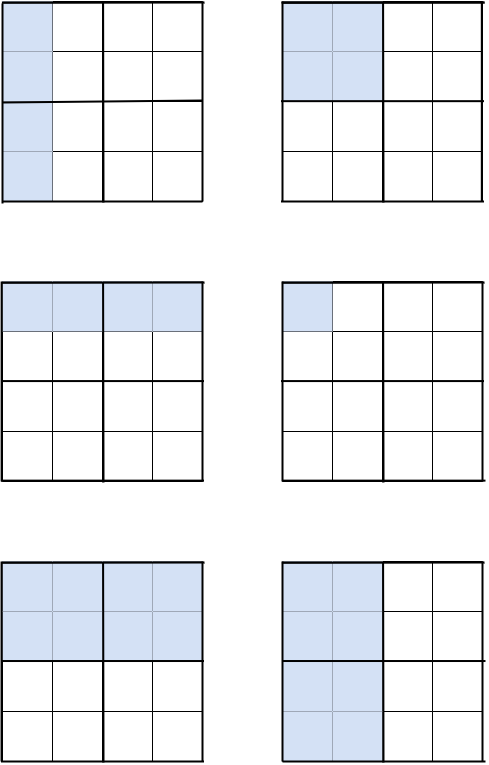
\includegraphics[width=50mm]{figures/highlighted_cells.png}
\end{center}
\caption{\label{fig:labels}From Left to Right, Top to Bottom. C1, B1, R1, cell (1,1), S1, T1 }
\end{figure}

% ~~~~~~~~~~~~~~~~~~~~~~~~~~~~~~~~~~~~~~~~~~~~~~~~~~~~~~~~~~~~~~~~~~~~~~~~~~~~~~~~~~~~~~~~~~~~ %
\chapter{Computational Complexity: Sudoku is Hard}

For this chapter the discussion is limited to sudokus of size $n \times n$ where $n$ is a square number.

Imagine a sudoku of size $m^2\times m^2$. How big does $m$ have to be for you to need more than a day to solve it? Maybe 6 or 10 or even just 4. Well turns out a computer cannot do large sudoku quickly either, or at least no one has found a quick algorithm yet. Currently, incrementing $m$ by 1 leads to an exponential increase in compute time and the most optimal algorithms for solving sudoku are infeasible for $100 \times 100$.

So, it is suspected that sudoku does not have a quick solution as there is no explicit method that computes a complete grid from a partial grid in reasonable time. This is not enough to convince mathematicians so it must be proven that a quick way does not exist. But proving something does not exist is a hard task, luckily there is a method in complexity theory to deal with this. When given a problem that is hard to solve, even for a computer, it is definitively called difficult if another known difficult problem can be transformed to this new problem. This chapter will discuss this in detail by defining what makes a problem difficult and then proving it for various problems that are all linked to sudoku. 

\section{A Complexity Theory Introduction}

This branch of theoretical computer science attempts to answer questions about the difficulty of problems and multiple types of difficulty. The focus in this chapter is on time complexity, the time taken for a problem to be solved, this is of course important as it allows differentiation between problems that take milliseconds to those that take generations. This is not often considered in pure mathematics as it contains many existence theorems that have non constructive proofs. Such as the Nash existence theorem in game theory, while it is proven a Nash equilibrium must exist there is no known algorithm to compute the equilibrium in a feasible amount of time \cite{ppad}.

\subsection{Turing Machines - An Abstract Computer}

The union of theoretical computer science and mathematics requires a rigorous definition of a computer, that's where the Turing Machine comes in. In Turing's paper \textit{Computing Machinery and Intelligence} \cite{turing} the Turing Machine is introduced as a mathematical model of what is now known as a CPU, the difference being that the theoretical machine has finite but unbounded memory. While the full definition isn't completely necessary for the discussion it is included for completeness.

\textbf{Def$^\text{n}$:} A \textbf{Turing Machine} is a tuple $M=(Q,\Gamma,b,\Sigma, \delta, q_0, F)$ such that:
\begin{itemize}
\item $Q$ a set of states, with $q_0\in Q$ the initial state and $F\subseteq Q$ the set of final states.
\item $\Gamma$ a finite alphabet of symbols, with $b\in \Gamma$ the blank symbol.
\item $\Sigma\subseteq \Gamma \symbol{92} \{b\}$ the set of input symbols
\item $\delta$ the set of transition functions, given the current state and symbol the transition function determines which state to progress to and whether to change the symbol, if the transition is undefined the machine halts.
\end{itemize}

The input is the original contents of the tape, and the output is the contents of the tape once the machine halts. A computable function is defined as a function that has an instance of a Turing machine with defined alphabet, states, and state transitions.

Consider a less tangible version of the Turing Machine one involving nondeterminism. When given a single state there may exist multiple transitions that can be taken. A non-deterministic Turing Machine explores all possible transitions at once by changing the set of state transitions $\delta$ from a function to a relation. 

\textbf{Def$^\text{n}$:} A \textbf{non-deterministic} Turing Machine is the mathematical model of a CPU that can undertake many actions in a single time step.

See figure \ref{ndtm} and figure \ref{dtm} for a comparison between these two versions of Turing machines when solving a 4 by 4 sudoku with a brute force method. Each row executes in the same time step.

\begin{figure}[h!]
\begin{center}
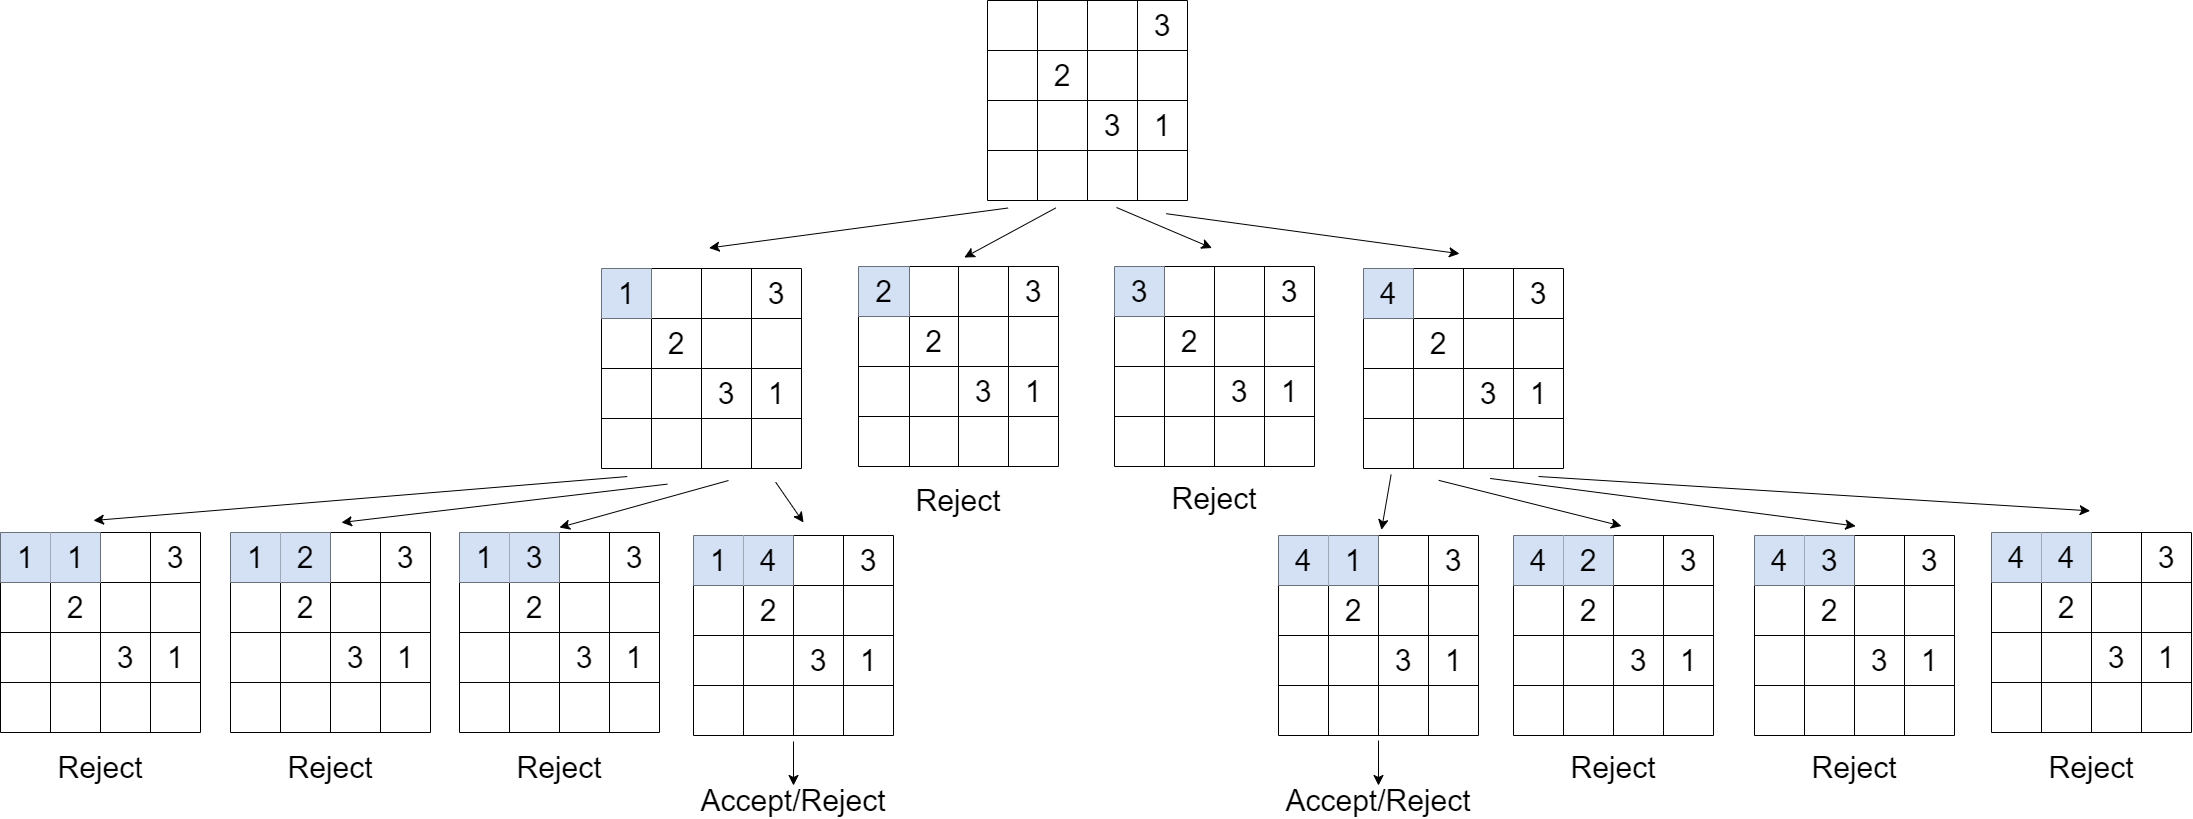
\includegraphics[width=180mm]{figures/turing_non_determinism.png}
\end{center}
\caption{\label{ndtm} Non Deterministic Turing Machine with Brute Force Solving}
\end{figure}

\begin{figure}[h!]
\begin{center}
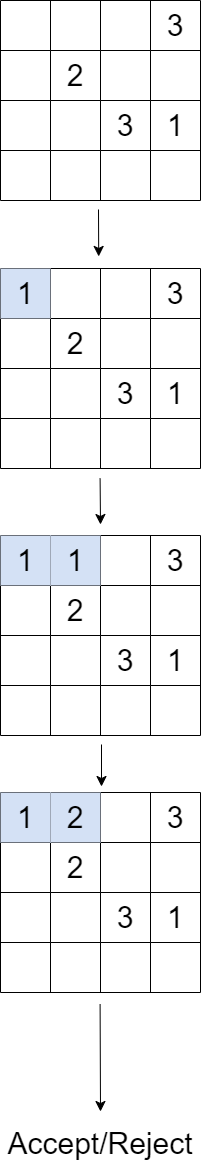
\includegraphics[width=18mm]{figures/turing_determinism.png}
\end{center}
\caption{\label{dtm} Deterministic Turing Machine with Brute Force Solving}
\end{figure}

\subsection{Big O Notation}

In the real-world computers come in all shapes and sizes and with this take different amounts of time to execute an instruction. This leads to difficulty when defining time complexity as a supercomputer may execute a task in a minute when a laptop may take a day. In order to remove this ambiguity from complexity theory time is taken to mean the number of steps a computer performs over actual temporal associations. A step is then defined as a small action made by a computer such as a comparison or an addition. 

The abstractions go further, time complexity does not care for constant terms as an algorithm taking $n$ steps and another with $2n+5$ steps are similar in difficulty. The following notation enables this abstraction.

\textbf{Def$^\text{n}$:} Let $f$ be a function indicating the amount of steps take in the execution of an algorithm and $g$ a strictly positive function. $f(x)=O (g(x))$ if $\exists$ positive $ M$ and $x_0$ such that $|f(x)|\leq Mg(x)$ $\forall$ $x\geq x_0$. This is coined \textbf{Big O Notation}.\footnote{Chapter 2 of \cite{salomaa1985computation} has a application based discussion of Big O.}

\textbf{Properties:} Following from the definition is some immediate properties, assume $f,g,h,i$ are functions obeying the necessary conditions of the definition.
\begin{itemize}
\item Product: $f=O(g)$ and $h=O(i)$, $fh=O(gi)$.
\item Sum: for $f=O(g)$ and $h=O(i)$, $f+h = O(max(g,i))$.
\item Constant Multiplication: for constant $k\neq0$, $O(kg)=O(g)$.
\end{itemize}

The properties of big O notation confirm its ability to abstract away constant terms as was required. Big O is our measure of time in complexity theory. With this abstract further into classes of time such as constant, linear, polynomial, and exponential. A definition of polynomial time is below but the rest are omitted until the example section as they are self-explanatory.

\textbf{Def$^n$:} A polynomial time algorithm is an algorithm with $O(x^c)$.

\subsection{Sets of Difficulty} 

So there exists a computer and a measure of execution time but still no difficulty. To define difficulty no measure is created instead there are sets. These sets are defined on decision problems. These are problems that given an input produce a 'yes' or 'no' answer. There exist many sets of these problems.

\begin{itemize}
\item{P (Polynomial) is the class of problems that can be solved in polynomial time by a deterministic Turing machine.}
\item{NP (Non-deterministic Polynomial) is the class of problems that can be verified in polynomial time by a deterministic Turing machine or solved in polynomial time by a non-deterministic Turing machine.}
\item{the NP-hard class are at least as hard as the hardest NP problem;} 
\item{the NP-complete set is the intersection of NP and NP-hard problems, these are the hardest problems in NP;} 
\item{the coNP class if the complement of all NP problems, for each problem in NP there exists a problem in coNP but 'yes' and 'no' instances are reversed.}
\end{itemize}

For a visualisation of these sets see figure \ref{fig:npsets}.

Problems in P are considered feasible and those in NP-complete are infeasible as their complexity scales exponentially with respect to the input size and as it is assumed they cannot be solved in polynomial time ($P \neq NP$).\footnote{$P\neq NP$ is only assumed as this problem is yet to be proven, it is in fact one of the Millennium Prize problems.} Anything above polynomial time takes too long from complexity theory's point of view.

So, when saying sudoku is hard this actually means sudoku belongs to NP-complete. Sudoku cannot be just proven to belong to NP as this also includes problems in P, it must be proven to be one of the hardest problems in NP.\footnote{Due to Ladner's Theorem there exists problem $\in$ NP but $\not\in$ NP-complete and $\not\in$ P iff $P\neq NP$, these problems are called NP-intermediate.}

\begin{figure}[h!]
\begin{center}
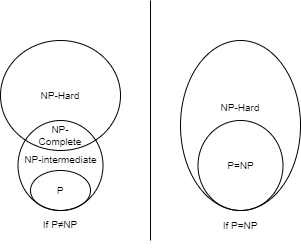
\includegraphics[width=70mm]{figures/np.drawio.png}
\end{center}
\caption{An illustration of complexity sets P, NP, NP-complete \& NP-hard sets\label{fig:npsets}}
\end{figure}

\subsection{Proving NP Completeness}

If a problem is NP-complete it is difficult but how does one show that a problem belongs to this class? 

Call the problem $x$.

The set of NP-complete problems are defined as members of both the set of NP problems and the set of NP-hard problems. 

First show there exists a verifier for $x$ with a polynomial or less runtime, this is a algorithm that decides if a proposed solution to problem $x$ is correct. This proves $x\in$ NP.

The hard part comes from showing $x\in$ NP-hard. The NP-hard class is defined as at least as hard as the hardest NP problem, this requires a comparison between problems. Problems can be compared to each other through a reduction as follows.

\noindent\rule{4cm}{0.4pt}

\textbf{Def$^\text{n}$:} A \textbf{Reduction}, $A \leq_p B$, is a transformation in polynomial time ($O(x^c)$) from problem set $A$ to problem set $B$. The converse applies for $A\geq_p$B; there exists a transformation in polynomial time from $A$ to $B$.

\begin{figure}[h!]
\begin{center}
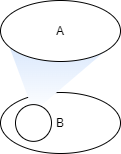
\includegraphics[width=30mm]{figures/reduction.png}
\end{center}
\caption{\label{fig:reduction}A$\leq_p$B}
\end{figure}

This author finds the reduction concept to be understood best when visualised as in figure \ref{fig:reduction}. The transformation (represented by the blue funnel) takes all problems in $A$ and maps them to a corresponding problem in $B$ such that all the transformed $A$ is now a subset of $B$. From this perspective the similarities between $\leq$ and $\leq_p$ are more apparent as the set of $B$ will always be as large or larger than $A$, it can even be thought of as a difficulty comparison of $A\leq_p B$ is the same as saying $B$ is as difficult as $A$ or has greater difficulty.

This comparison notion allows the proof to be completed.

\noindent\rule{4cm}{0.4pt}

So take a known NP-complete problem call this $y$, and reduce it to $x$, one does this by transforming the input of $y$ to the input of $x$ in polynomial time, call this function $g: y\rightarrow x$. Assume there exists a polynomial time algorithm to solve $x$, $f$, then $y$ coule be solved in polynomial time too, $f(g(y))$. If the reduction exists then $x$ is at least as hard as $y$ and as $y$ is NP-hard then $x$ is at least as hard as the hardest question in NP meaning $x \in$ NP-hard.

Therefore, $x\in $ NP-complete.

\subsection{The First NP-complete Problem} 

If, as the above suggests, an NP-complete problem is required to prove a problem is NP-complete then a stalemate has been reached. Luckily there is the Cook-Levin Theorem.

\textbf{Cook-Levin Theorem}\cite{compcomplexityamodernapproach}: SAT is NP-Complete.

This introduces a new problem named SAT, to understand the problem some terminology must be introduced.

\textbf{Terminology}:
\begin{itemize}
\item Boolean variable: a variable that can be true or false ($a=T$ or $a=F$).
\item Literal: a boolean variable or it's negation (if $a = T$ then its negation $\neg a = F$).
\item $\land$: an operation that outputs true when all operands are true, false otherwise ($a\land b = T$ iff $a=T$ and $b=T$).
\item $\lor$: an operation that outputs true when at least one operand is true, false otherwise ($a\lor b = F$ iff $a=F$ or $b=F$).
\item Clause: multiple literals operated on by $\lor$s, a set of clauses are joined by $\land$s.
\item Truth Assignment: assignment of true and false values to each boolean variable. 
\end{itemize}

\textbf{Def$^n$}: SAT is the following decision problem. Given a set of boolean variables $B$ and a collection of clauses $C$ does a valid truth assignment exist that satisfies all clauses in $C$?

Given $B = \{a,b,c\}$ and $C=\{(a\lor b \lor c \lor \neg c), (a \lor c), (\neg a\lor b)\}$ a valid truth assignments exists. See the table \ref{satex} for all valid assignments.

\begin{table}
\begin{center}
\begin{tabular}{ |c|c|c|c|c|c|c| }
\hline
\multicolumn{7}{|c|}{$(a\lor b \lor c \lor \neg c)\land (a \lor c) \land (\neg a\lor b)$} \\
\hline
$a$ & $b$ & $c$ & $(a\lor b \lor c \lor \neg c)$ & $(a \lor c)$ & $(\neg a\lor b)$ & Full Clause\\
\hline
F & F & F & T & F & T & F \\
\rowcolor{lightgray}
F & F & T & T & T & T & T \\
F & T & F & T & F & T & F \\
\rowcolor{lightgray}
F & T & T & T & T & T & T \\
T & F & F & T & T & F & F \\
T & F & T & T & T & F & F \\
\rowcolor{lightgray}
T & T & F & T & T & T & T \\
\rowcolor{lightgray}
T & T & T & T & T & T & T \\
\hline
\end{tabular}
\end{center}
\caption{\label{satex}An example of a SAT clause set with all possible truth assignments explored and valid assignments highlighted.}
\end{table}

Now there is an NP-complete problem to reduce the sudoku problem to.

\subsection{Examples}

Before the proof of sudoku's complexity it is important to understand complexity theory in the context of sudoku with example algorithms. The input is a puzzle $p$ of size $n\times n$ ($n=m^2$), the algorithm's run time is a function of this variable.

\textbf{Constant time, $O(1)$:} This includes functions that take the same time no matter the input size, for example accessing the value of a cell in the sudoku grid, even as the puzzle increases in size, $p(x,y)$ takes constant time.

\textbf{Linear time, $O(n)$:} Consider a function that when given a puzzle and a cell $(x,y)$ outputs a boolean value; true if the value of the puzzle at this cell is valid (does not repeat in the row, column or box) and false otherwise. Consider the inner workings of the function: 
\begin{itemize}
\item First assume the comparison between two values takes a single unit of time $O(1)$
\item A comparison of the value at the given cell with each value on the row must be made, observe this is performed $n-1$ times and therefore this operation takes $O(n)$ time.
\item Then compare the value at the given coordinate with each value on the column, as per the previous argument this has complexity $O(n)$.
\item Finally compare the value with the remainder of the box value that have not been compared previously, this takes $n-(\sqrt{n}-1)-(\sqrt{n}-1)-1= n-2\sqrt{n}+1$ comparison operations which has a complexity of $O(n)$.
\end{itemize}
Overall this function takes $(n-1)+(n-1)+(n-2\sqrt{n}+1) = 3n -2\sqrt{n}-1$ comparisons and therefore calculates the boolean variable in linear time ($O(n)$). See algorithm \ref{alg:validentry}.

\begin{algorithm}
\caption{Validate an Entry\label{alg:validentry}}
\begin{algorithmic}
\Procedure{ValidateEntry}{$p$, $(x,y)$, $n$}
\For{$i$ = 1 to $n$} \Comment{Check column}
\If{$i \neq x$}
\If{$p(i,y) = p(x,y)$}
\State{return False}
\EndIf
\EndIf
\EndFor
\For{$i$ = 1 to $n$} \Comment{Check row}
\If{$i \neq y$}
\If{$p(x,i) = p(x,y)$}
\State{return False}
\EndIf
\EndIf
\EndFor
\For {$(i,j)\in$ B$k$ where $(x,y)\in$B$k$} \Comment{Check box}
\If {$p(i,j) = p(x,y)$} 
\State{return False}
\EndIf
\EndFor
\State{return True}
\EndProcedure
\end{algorithmic}
\end{algorithm}

\textbf{Polynomial time, $O(n^t)$}: Consider a function that when given a partially complete sudoku grid returns true if the grid is valid, otherwise returns false. Using the linear time algorithm just described repeated it for every value within the grid. See algorithm \ref{alg:valid}.

\begin{algorithm}
\caption{Validate a Grid\label{alg:valid}}
\begin{algorithmic}
\Procedure{Validate}{$p$, $n$}
\For{$i$ = 1 to $n$} \Comment{Loop through all $(i,j)$ pairs to validate all squares of the grid}
\For{$j$ = 1 to $n$ }
\If{ValidateEntry($p$, $(i,j)$, $n$) = False}
\State{return False}
\EndIf
\EndFor
\EndFor
\State{return True}
\EndProcedure
\end{algorithmic}
\end{algorithm}

ValidateEntry is called $n^2$ times so the complexity is $O(n\times n^2) = O(n^3)$ this is polynomial and therefore still considered feasible as $n$ increases. 
\textbf{Exponential time, $O(a^n)$}: Consider a brute force algorithm to solve sudoku. Cycle through values 1 to $n$ for all cells rejecting those that create an invalid sudoku grid and outputting a valid grid if one is found, otherwise false if the sudoku cannot be solved. See algorithm \ref{alg:bruteforce}.

\begin{algorithm}
\caption{Brute Force Sudoku Solver\label{alg:bruteforce}} 
\begin{algorithmic}
\Procedure{BruteForceSolve}{$p$, $n$}
\If{$p$ is complete}
\If{Validate($p$) = True}
\State{return $p$}
\Else
\State{return False}
\EndIf
\EndIf
\State{(x,y) = location of first empty cell in grid}
\For{$i$ = 1 to $n$}
\State{$p(x,y) = i$}
\If{BruteForceSolve($p$, $n$) $\neq$ False}
\State{return $p$}
\EndIf
\EndFor
\State{return False}
\EndProcedure
\end{algorithmic}
\end{algorithm}

This algorithm refers to itself, this is called recursion and shall be explored further in chapter 4 when other solving techniques are discussed. The complexity is computed as follows. 
\begin{itemize}
\item Assume there is only 1 empty cell. Try the values 1 to $n$ and for each check if the grid is valid, this takes $O(n\times n^3)$.
\item Now assume there is 2 empty cells, try 1 to $n$ and for every option do the same as the first bullet point which takes $O(n\times n \times n^3)$.
\item A pattern forms, for every empty square times the complexity by $n$, there are at most $n^2$ empty squares so the upper bound is $O(n^{n^2+3})$.
\end{itemize}
This algorithm has a complexity that is a bit above exponential as the base is dependent on $n$ too however it is not quite factorial complexity, so it is called exponential. This is infeasible for large values of $n$ and does not belong to P. So, solving sudoku is hard, case closed - not quite, this is only one example of a sudoku solver there may exist more efficient algorithms so this needs to be disproved. \footnote{BogoSort is a sorting algorithm that randomises a list until it is in the correct order, this has an unbounded run time, but there exists sorting algorithms with complexity $O(n\text{log}n)$. See Chapter 4 of \cite{heineman2016algorithms} for a thorough discussion of sorting algorithms.} 

%%%%%%%%%%%%%%%%%%%%%%%%%%%%%%%

\section{Existence is Hard}
Now onto the proof, define the decision problem:

\begin{equation}
\Phi (p) = \begin{cases}
\text{True if a completion exists} \\
\text{False if a completion does not exist}.
\end{cases}
\end{equation}

The question is does there exist a function $\Phi$ that when given an instance of the problem will, in polynomial time or less,
return True if it can be solved and False otherwise.

\noindent\rule{4cm}{0.4pt}

\textbf{Proof Outline}

The verifier must be shown to be $\in$ P, this means the Sudoku decision problem belongs to the set NP. Then a reduction from sudoku to a known NP-complete problem proves sudoku is also NP-hard. A chain of reductions will be used to simplify the reduction process: \textbf{Sudoku $\geq_p$ Latin Square $\geq_p$ Triangulated Tripartite $\geq_p$ 3SAT $\geq_p$ SAT}. This chain can be seen in figure \ref{fig:sudokureduction}, this visualisation emphasises the direction of the reduction as it is important that the set of sudoku problems has 3SAT as a subset (achieved through the transitivity of sets). If it is possible to solve all sudoku problems and 3SAT transforms to a subset of sudoku then it is intuitive that it is possible to solve 3SAT. The same cannot be said if sudoku was transformed to a subset of 3SAT as being able to solve sudoku does not help with the 3SAT problems existing outside of the sudoku transformation subset. Once this is proven the Sudoku decision problem is a member of NP and NP-hard it is NP-complete by definition.

\begin{figure}[h!]
\begin{center}
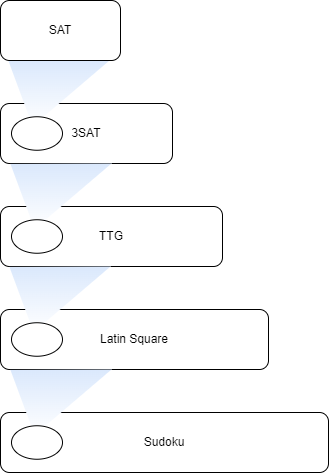
\includegraphics[width=80mm]{figures/subset.png}
\end{center}
\caption{\label{fig:sudokureduction}}
\end{figure}

\textbf{Note}: Theoretically any problem in the set NP-complete can be reduced to Sudoku and therefore this reduction is not unique, however, it is the most intuitive way. Some readers may question why the reduction to Graph Colouring is not being used problem but later in this chapter it is shown this is the wrong direction of reduction.

%%%%%%%%%%%%%%%%%%%%%%%
\subsection{Verification is Easy}

Given a sudoku grid $p$, there exists an algorithm to determine:
\begin{equation}
\Psi(p) = \begin{cases} 
\text{True if the puzzle is complete} \\
\text{False if the puzzle is not complete}.
\end{cases}
\end{equation}
This algorithm is an extension of algorithm \ref{alg:valid} from the complexity examples, simply add a for loop to the end to check that $\forall S(i,j) \neq 0 $, in other words there are no empty cells. To find the complexity algorithm add $n^2$ to the complexity of the original validation algorithm, giving $O(n^2+n^3)=O(n^3)$. This is polynomial time, therefore $\Psi\in $P.
%%%%%%%%%%%%%%%%%%%%%%%
\subsection{Sudoku $\geq_p$ Latin Square}

\textbf{Def$^n$}: A valid Latin Square puzzle is a function $L:i,j \rightarrow x$ for values $i,j \in \{1,..,D\} $ and $x \in
\{0,...,D\}$ satisfying the following:
\begin{itemize}
\item{for all $a,b,c \in \{1,...,D\}$ with $L(a,b) \neq 0 $ and $L(a,c) \neq 0$ then $L(a,b) \neq L(a,c)$}
\item{for all $a,b,c \in \{1,...,D\}$ with $L(a,b) \neq 0 $ and $L(c,b) \neq 0$ then $L(a,b) \neq L(c,b)$}
\end{itemize}
It is complete or solved if for all $i,j \in \{1,...,D\}$, $L(i,j) \neq 0$.

\textit{What is the Latin Square decision problem?} Given a Latin square puzzle $L$, can the function be augmented, by changing only the value of the function for value pairs $i,j$ that previously gave $L(i,j) =0$, to get a complete Latin square puzzle?

\noindent\rule{4cm}{0.4pt}

\textit{Proof idea:} Reduce a given Latin square grid of size $D \times D$ to a sudoku grid size $D^2 \times D^2$ that is solvable if and only if the Latin square is.

\textbf{Lemma:} (from \cite{sls}) let $S_l$ be a Sudoku problem with the following construction 
\begin{equation}
S_l(i,j) =\begin{cases}
0 \qquad\qquad\qquad\qquad\qquad\qquad\text{when } (i,j) \in L_s \\ 
((i-1 \text{ mod } n)n + \left\lfloor{i-1/n}\right\rfloor+j-1)\text{ mod } n^2 +1 \quad\text{otherwise}
\end{cases}
\end{equation}
where $L_s=\{(i,j)| \left\lfloor{i-1/n}\right\rfloor=0 \text{ and }(j \text{ mod }n)=1\}$. Then there exists an augmentation $S_l'$ to complete the sudoku puzzle if and only if the square $L$ such that $L(i,j/n)=S_l'(i,j)-1/n+1$ for all $(i,j) \in L_s$ is a Latin square.

Figure \ref{formula} gives examples of generated sudokus from this formula.

\begin{figure}[h]
\centering
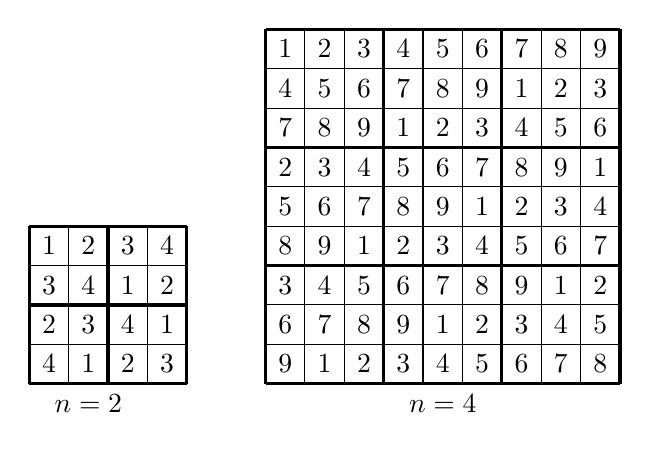
\begin{tikzpicture}[scale=.5]
\begin{scope}[xshift=10cm]
\draw (0, 0) grid (4, 4);
\draw[very thick, scale=2] (0, 0) grid (2, 2);
\setcounter{rowa}{1}
\setrowa {1}{2}{3}{4}
\setrowa {3}{4}{1}{2}
\setrowa {2}{3}{4}{1}
\setrowa {4}{1}{2}{3} 
\node[anchor=center] at (1.5, -0.5) {$n=2$};
\end{scope}
\begin{scope}[xshift=16cm]
\draw (0, 0) grid (9, 9);
\draw[very thick, scale=3] (0, 0) grid (3, 3);
\setcounter{row}{1}
\setrow {1}{2}{3} {4}{5}{6} {7}{8}{9}
\setrow {4}{5}{6} {7}{8}{9} {1}{2}{3}
\setrow {7}{8}{9} {1}{2}{3} {4}{5}{6}
\setrow {2}{3}{4} {5}{6}{7} {8}{9}{1}
\setrow {5}{6}{7} {8}{9}{1} {2}{3}{4}
\setrow {8}{9}{1} {2}{3}{4} {5}{6}{7}
\setrow {3}{4}{5} {6}{7}{8} {9}{1}{2}
\setrow {6}{7}{8} {9}{1}{2} {3}{4}{5}
\setrow {9}{1}{2} {3}{4}{5} {6}{7}{8}
\node[anchor=center] at (4.5, -0.5) {$n=4$};
\end{scope}
\end{tikzpicture}
\caption{Formula Generation of Valid Sudoku}
\label{formula}
\end{figure}

\textit{Proof:}

First show $S_l(i,j)=((i-1 \text{ mod } n)n + \left\lfloor{i-1/n}\right\rfloor+j-1)\text{ mod } n^2 +1$ forms a complete and valid sudoku puzzle.

When $i=[1,...,n^2]$ then:
\begin{align}
0&<\left\lfloor{i-1/n}\right\rfloor<n-1\\
0&<i-1 \text{ mod } n<n-1\\
0&<(i-1 \text{ mod } n)n + \left\lfloor{i-1/n}\right\rfloor<n^2-n\\
0&<(i-1 \text{ mod } n)n + \left\lfloor{i-1/n}\right\rfloor+j-1<n^2-1\\
1&<((i-1 \text{ mod } n)n + \left\lfloor{i-1/n}\right\rfloor+j-1)\text{ mod } n^2 +1<n^2\\
1&<S_l(i,j)<n^2
\end{align} 
Note $\left\lfloor{i-1/n}\right\rfloor$ gives the row coordinate when indexed at 0 in which the larger box that (i,j) belongs to starts and $i-1 \text{ mod } n$ gives the row within that box when indexed at 0. Therefore $(\left\lfloor{i-1/n}\right\rfloor,i-1 \text{ mod } n)$ will take all value pairs of integers between 0 and $n-1$.

When j is fixed (particular column), assume two cells have the same value, that is $S_l(i,j)=S_l(i',j)$ then
\begin{align}
(i-1 \text{ mod } n)n + \left\lfloor{i-1/n}\right\rfloor+j-1 &= (i'-1 \text{ mod } n)n +
\left\lfloor{i'-1/n}\right\rfloor+j-1\\
(i-1 \text{ mod } n)n + \left\lfloor{i-1/n}\right\rfloor &= (i'-1 \text{ mod } n)n + \left\lfloor{i'-1/n}\right\rfloor
\end{align}
from the above $i=i'$. No cell on a column has the same value.

When i is fixed (particular column) assume two cells have the same value, that is $S_l(i,j)=S_l(i,j')$ implies $j-1=j'-1 (\text{mod }n)$ therefore $j=j'$.

For the third condition fix $\left\lfloor{i-1/n}\right\rfloor$. (i-1 \text{ mod } n,j) takes all value pairs of integers 0 to n-1 so if a cell has the same value as another within the n by n square $S_l(i,j)=S_l(i',j')$ implying $(i-1 \text{ mod }n,j)=(i'-1 \text{ mod } n,j')$ which means $i=i'$ and $j=j'$. Therefore $S_l$ is a valid and complete sudoku puzzle.

Now consider which integers fill the blanks in $L_s$. For $(i,j)\in L_s$, $S_l(i,j)-1= ((i-1 \text{ mod } n)n+j-1)\text{ mod } n^2$ as $j \text{ mod } n=1$, $j-1\text{ mod }n=0$ therefore $S_l(i,j)-1$ is divisible by n so $S_l-1/n+1$ gives integers between $[1,...,n]$.
Therefore $L(i,j) \in [0,...,n]$.

Now to validate the Latin square conditions. The row constraint in $S_l$ ensures $S'(i,j)=S'(i,j') \implies j=j'$, $S'(i,j)-1/n+1=S'(i,j')-1/n+1 \implies j=j'$, $L(i,j/n)=S'(i,j'/n) \implies j=j'$ is equivalent to the row constraint of L. The column constraint of $S_l$ is equivalent to the column constraint of L. The small square constraint of $S_l$ is equivalent to the column constraint of L. $\square$

\subsection{Latin Square $\geq_p$ Triangulate A Tripartite Graph}

\textbf{Def$^n$}: A graph $G=(V,E)$ is tripartite if a partition $V_1$, $V_2$, $V_3$ exists such that the vertices are split into three sets with no edges between vertices that belong to the same set, i.e for all $(v_i,v_j) \in E\text{ if } v_i \in V_i\text{ then }v_j \not\in V_i $.

\textbf{Def$^n$:} A triangulation T of a graph is a way to divide edges into disjoint subsets $T_i$, each forming a triangle ($T_i=\{(v_{1}, v_{2}),(v_{2}, v_{3}),(v_{3},v_{1})\}$).

If a tripartite graph can be triangulated it must be uniform, that is: every vertex in $V_1$ (or $V_2$ or $V_3$) has the same number of neighbours in $V_2$ and $V_3$ (or the respective sets).

\textit{What is the Triangulated Tripartite decision problem?} Given a graph G that is tripartite (can be split into 3 subgroups, within these subgroups vertices should not share edges) can it be triangulated?

\noindent\rule{4cm}{0.4pt}

\textbf{Theorem:} (from \cite{lsttg}) completing a Latin square with dimensions n by n is equivalent to triangulating a tripartite graph $G= V_1, V_2, V_3$.

\textit{Proof:} 

Intuitively, a graph is mapped to a Latin square $L$ through the following: 
given tripartite graph G=(V,E) label vertices in $V_1$ with distinct labels $\{r_1,...r_n\}$, label vertices in $V_2$ with distinct labels $\{c_1,...c_n\}$ and label vertices in $V_3$ with distinct labels $\{e_1,...e_n\}$. Add edges such that:
\begin{itemize}
\item{If $L(i,j) = 0$ then add the edge $(r_i,c_j)$ }
\item{If for all $i \in [0,...,n]$ and constant j, $L(i,j) \neq k$ then add the edge $(r_i,e_k)$}
\item{If for all $j \in [0,...,n]$ and constant i, $L(i,j) \neq k$ then add the edge $(c_j,e_k)$}
\end{itemize}
This graph has a triangulation if and only if $L(i,j)$ can be solved.

Now show every uniform tripartite graph can be transformed to the above formulation of a Latin square.

\begin{figure}[h!]
\centering
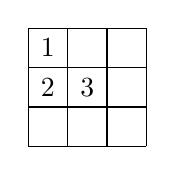
\begin{tikzpicture}[scale=.5]
\begin{scope}[xshift=10cm]
\draw (0, 0) grid (3, 3);
\setcounter{rowb}{1}
\setrowb {1}{}{}
\setrowb {2}{3}{}
\setrowb {}{}{}
\end{scope}
\end{tikzpicture}

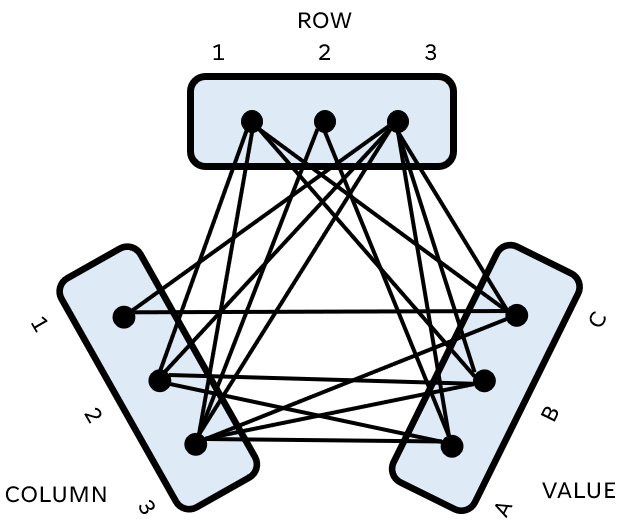
\includegraphics[height=40mm]{figures/ttg.png}
\caption{The Latin Square is equivalent to the Tripartite Graph.}
\end{figure}

First a generalisation of a Latin square is required.

\textbf{Def$^n$}: A Latin framework LF for tripartite graph G, size (r,s,t) is a r by s array with values [1,...,t]. With constraints:
\begin{itemize}
\item{Each row/column contain each element only once.}
\item{If $(r_i,c_j)\in E$ then LF(i,j)=0 else LF(i,j)= k, $k\in [1,...,t]$}
\item{If $(r_i,e_k)\in E$ then $\forall j$ $LF(i,j)\neq k$}
\item{If $(c_j,e_k)\in E$ then $\forall i$ $LF(i,j)\neq k$}
\end{itemize}
If r=s=t then LF is a Latin square (formulation above) which can be completed if and only if G has a triangle partition.

\textbf{Lemma}: For tripartite graph G=(V,E) with $|V_1|=|V_2|=|V_3|=n$ (uniform), there's a Latin framework of (n,n,2n).

\textit{Define LF an n by n array. For $(r_i,c_j)\in E$ $LF(i,j)=0$ else $LF(i,j)=1+n+((i+j)\text{ mod }n)$. LF is a Latin framework as the first two bullet points of the definition hold by construction and as $1+n\leq LF(i,j)\leq 2n$ LF will never equal a value in $1,...n$ and therefore the last two bullet points hold. The size is trivial. $\square$}

\textbf{Lemma}: Given Latin framework $LF(n,n,2n)$ for uniform tripartite graph G, this can be extended to have size $(n,2n,2n)$.

\textit{First have a few notations: R(k) = the number of times k appears in L plus half $|e_k|$; $S_i=\{k|k \not\in LF(i,j)\forall j$ $ \cap$ $ (r_i,e_k)\not\in E\}$; $M=\{k|R(k)=r+s-t\}$. Show sets $S_1,...S_r$ have a system distinct representative containing all elements of $M$, then add this system as the $(s+1)$st column and repeat until there are $2n$ columns.}

\textit{Using Hoffman and Kuhn's theorem \cite{hoffman} it is only necessary to show that $S_1,...S_r$ have a system distinct representative and that for every $M'\subseteq M$ at least $|M'|$ of sets $S_1,...S_r$ have non empty subsections with $M'$.}

\textit{First choose any $m$ sets such that $1\leq m \leq r$. As G is uniform each set has t-s elements, so $m$ sets together have $m(t-s)$ cardinality. Each value $1,...,t$ appears at least r+s-t times in $LF$, so note each value appears in at most $t-s$ of the sets $S_i$. Consider the union of the $m$ sets, this contains some $p$ elements so $p(t-s)\geq m(t-s)$ therefore $p\geq m$. So any $m$ sets have at least $m$ elements in their union and by Hall's theorem \cite{hall} a system distinct representative exists.}

\textit{Next take $M'\subseteq M$ and assume there are $p$ sets in $S_1,...S_r$ that have a nonempty intersection with $M'$. Each set has $t-s$ elements and together have cardinality $p(t-s)$, each element of $M$ appears in exactly $r-(r+s-t)=t-s$ of the $s_i$s, therefore $|M'|(t-s)\leq p(t-s)$ so $|M'|\leq p$. At least $|M'|$ sets have nonempty intersections with $M'$.}

\textit{The Hoffman and Kuhn theorem holds and therefore a system distinct representative exists and can be added to the end. Repeat this n times.} $\square$

\textbf{Lemma}: Latin framework (n,2n,2n) for graph G, can be extended to (2n,2n,2n).

\textit{Transpose the array and do the same as the previous lemma. $\square$}

\textbf{Note}: Find a system distinct representative using the Hopcroft-Karp \cite{hopcroft} algorithm which solves bipartite matching in polynomial time. 

Given a tripartite graph G, if it is not uniform then no triangulation exists, else apply the above to produce a Latin framework of size (2n,2n,2n) in polynomial time. This is a Latin square which can be completed if and only if G has a triangulation. The latin square problem has been reduced to the triangulating a tripartite graph problem. $\square$

\subsection{Triangulated Tripartite $\geq_p$ 3SAT}

\textit{What is 3SAT?} With a set of boolean variables $B$ and a collection of clauses $C$, with at most 3 literals (a literal is any $b \in B$ or its negation $\bar{b}$) in each, does a valid truth assignment exist that satisfies $C$?
\begin{equation}
\phi (C,B) = \begin{cases}
\text{True if a truth assignment exists} \\
\text{False if a truth assignment does not exist}.
\end{cases}
\end{equation}
This decision problem is therefore an enforced limitation of SAT as defined in the section Computational Complexity.

\noindent\rule{4cm}{0.4pt}

\textit{Proof:}

This reduction is a little trickier as it required the introduction of the Holyer graph $H$ from \cite{holyer}, this graph has the topology of torus.

\textbf{Def$^n$}: The Holyer graph $H_{3,p}$ is the set of vertices $V=\{(x_1,x_2,x_3)\in \mathbb{Z}_p^3 \| x_1+x_2+x_3 \equiv 0 (mod p)\}$ and an edge exists between vertices $(x_1,x_2,x_3)$ and $(y_1,y_2,y_3)$ if distinct i,j and k exist such that:
\begin{itemize}
\item $x_i\equiv y_i (\text{mod }p)$
\item $x_j\equiv y_j+1 (\text{mod }p)$
\item $x_k\equiv y_k-1 (\text{mod }p)$
\end{itemize}
See figure \ref{holyer} for an example.

\begin{figure}[h!]
\begin{center}
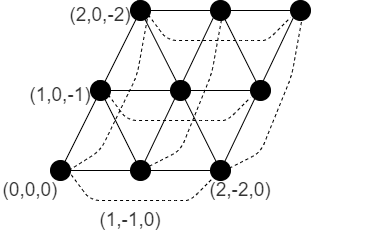
\includegraphics[height=40mm]{figures/holyer_coord.png}
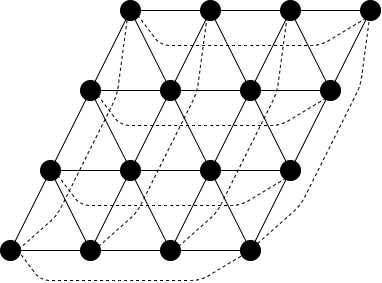
\includegraphics[height=40mm]{figures/holyer_3_4.png}
\end{center}
\caption{$H_{3,2} $ and $H_{3,3}$, the torus is embedded in the 2 dimensional plane, dotted lines link vertices that are the "same".}
\label{holyer}
\end{figure}

This graph is tripartite if and only if $p\equiv 0 $ (mod 3), this is demonstrated by a 3-colouring (a graph is tripartite if and only if it is 3-colourable) in figure \ref{holyercolour}.

\begin{figure}[h!]
\begin{center}
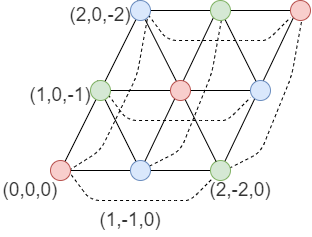
\includegraphics[height=40mm]{figures/colour_holyer_coord.png}
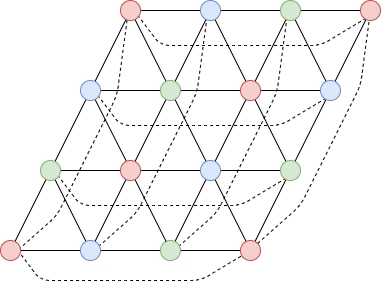
\includegraphics[height=40mm]{figures/colour_holyer.png}
\end{center}
\caption{3-colouring of $H_{3,2} $ and $H_{3,3}$ }
\label{holyercolour}
\end{figure}

\textbf{Def$^n$}: $H_{3,p}$ has only two triangulations, termed a true and a false triangulation, see figure \ref{truefalsetri}. 

\begin{figure}[h!]
\begin{center}
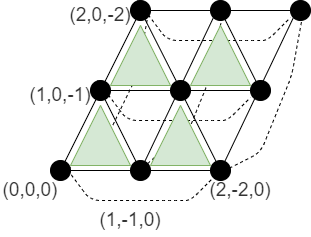
\includegraphics[height=40mm]{figures/holyer_true_triangulation.png}
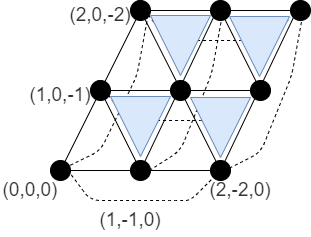
\includegraphics[height=40mm]{figures/holyer_false_triangulation.png}
\end{center}
\caption{True triangulation and a False triangulation on a $H_{3,2}$ graph. Notice the edges between (0,0,0), (1,0,-1) and (1,-1,0) uniquely determine the triangulation; if they belong to the same triangle then it is a true triangulation and false otherwise.}
\label{truefalsetri}
\end{figure}

\textbf{Note:} Connect graphs together by taking a set of vertices in $G_1$ and making them the 'same' as a set of vertices in $G_2$, sets are the same size.

\textbf{Def$^n$}: Graphs are connected with F-patches and T-patches, see figure \ref{patches}. 

\begin{figure}[h!]
\begin{center}
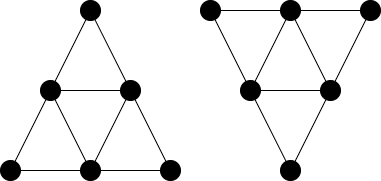
\includegraphics[width=70mm]{figures/patches.png}
\end{center}
\caption{F-patch and a T-patch}
\label{patches}
\end{figure}

Turn an instance of 3SAT into an instance of triangulating a tripartite graph through the following transformation process: (select p large enough to prevent patch overlap and $p\equiv 0 $ (mod 3))
\begin{itemize}
\item For $b_i\in B$ create $H_{3,p}$ called $G_{b_i}$.
\item For all $c_j\in C$, for each literal $l_{i,j}$ $j\in [1,2,3]$ create $H_{3,p}$ called $G_{i,j}$.
\item If $l_{i,j}=b_k$ connect an F-patch in $G_{b_k}$ to an F-patch in $G_{i,j}$, else if $l_{i,j}=\neg b_i$ connect a F-patch in $G_{i,j}$ to a T-patch in $G_{b_k}$.
\item For each $i$ connect one F-patch from each $G_{i,1}$, $G_{i,2}$ and $G_{i,3}$ then delete the centre triangle. 
\item $G = \{G_{b_i}$ $|$ $b_i \in B\}\cup\{G_{i,j}$ $|$ $ c_j\in C\text{ and }i\in [1,..,3] \}$
\end{itemize}
Now to prove the graph produced by this transformation can be triangulated if and only if there is a truth assignment satisfying the 3SAT formula.

Assume a triangulation of G exists, consider a H within the construction of G. H is either a true triangulation or a false triangulation. Now assume $l_{i,j}$ is $b_k$ and consider the join between $G_{i,j}$ and $G_{b_k}$ as this joins two F-patches to get at least one true triangulation: if $G_{i,j}$ is a true triangulation this accounts for all edges near the joining patch but the actual patch can be attributed to $G_{b_k}$ which can be triangulated either way; if both are false triangulations the connecting patch is forced to belong to both $G_{i,j}$ and $G_{b_k}$ which is a contradiction. (Figure \ref{holyerone})

\begin{figure}[h!]
\begin{center}
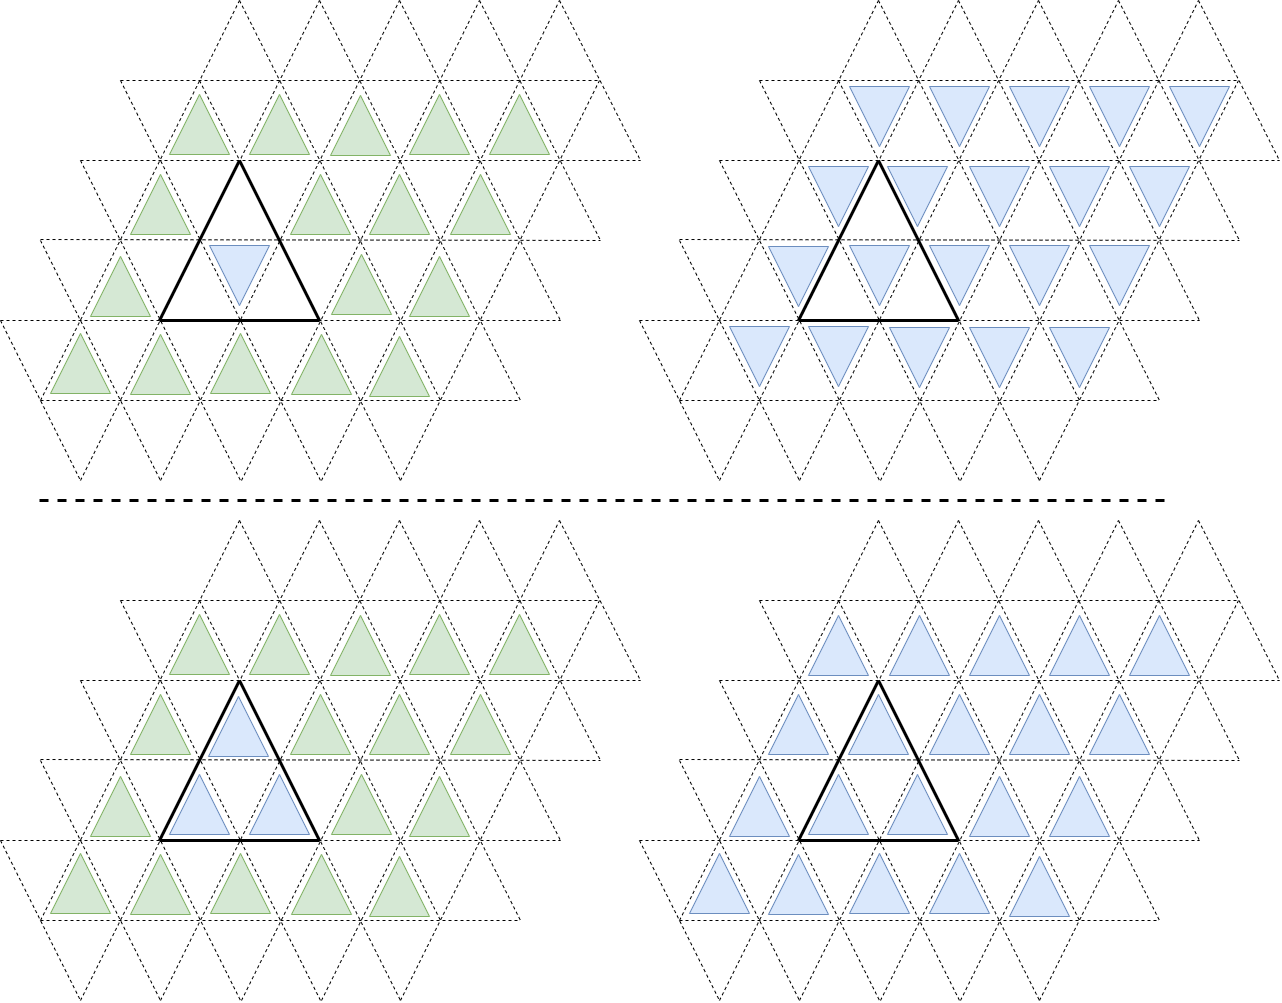
\includegraphics[width=100mm]{figures/first_holyer_lemma.png}
\end{center}
\caption{Graphs connected by two F-patches, the only complete triangulations are shown, one of each or two true triangulations.}
\label{holyerone}
\end{figure}


Similarly if $l_{i,j}=\neg b_i$ then $G_{i,j}$ is a false triangulation or $G_{b_k}$ is a true triangulation. (Figure \ref{holyertwo})

\begin{figure}[h!]
\begin{center}
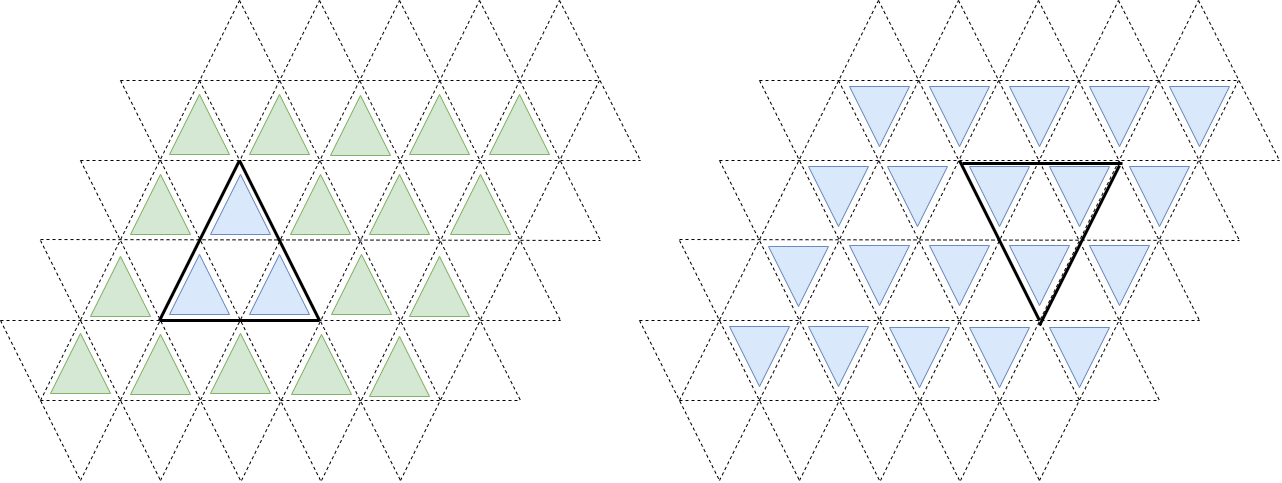
\includegraphics[width=100mm]{figures/lemma_two_holyer.png}
\end{center}
\caption{Graphs connected by a T-patch and a F-patch, the only complete triangulation is show.}
\label{holyertwo}
\end{figure}

Next the join between clause graphs allow for one false triangulation and the rest are true triangulations. As the centre of the patch is missing a single $G_{i,j}$ must take the outer edges of the patch by being a false triangulation. (Figure \ref{holyerthree})

\begin{figure}[h!]
\begin{center}
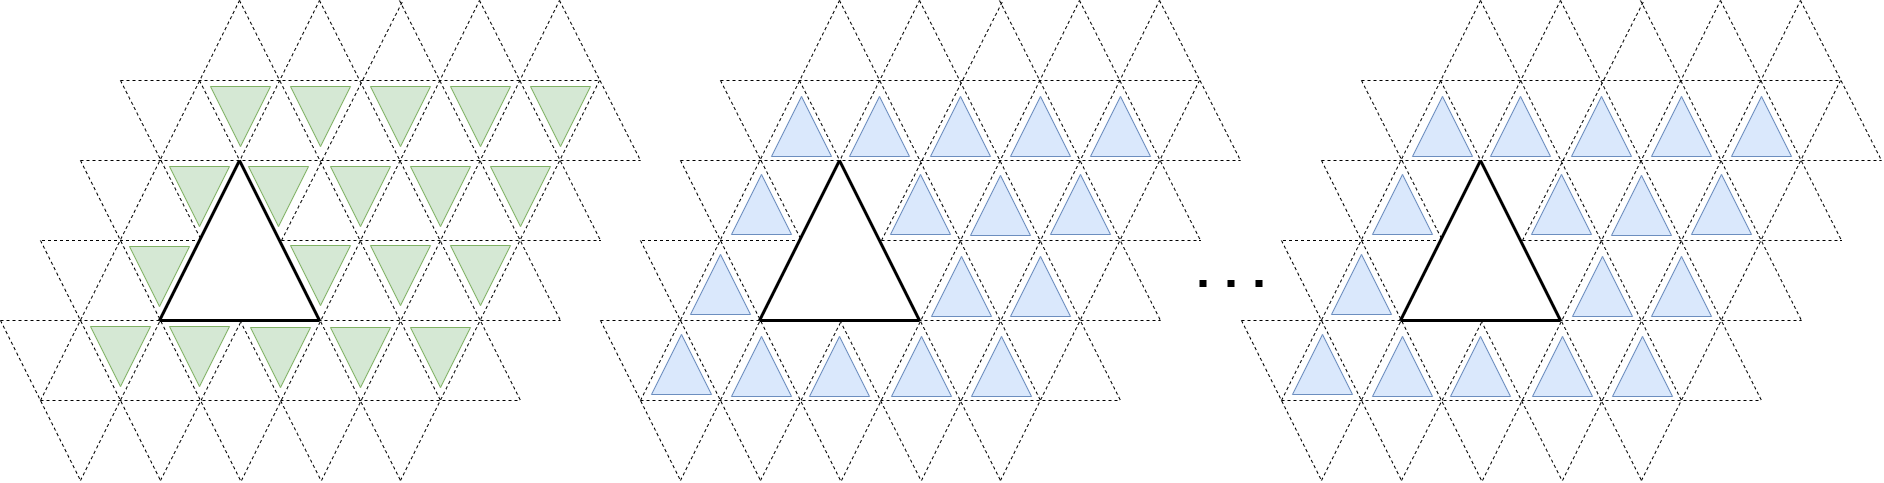
\includegraphics[width=120mm]{figures/lemma_three_holyer.png}
\end{center}
\caption{Graphs connected by F-patches with the centre removed, the only complete triangulation is show, exactly one must be a false triangulation.}
\label{holyerthree}
\end{figure}

If G can be triangulated a truth assignment exists such that variable $b_k$ is true if $G_{b_k}$ has a true partition otherwise it is false.

If there exists a truth assignment $G_{b_k}$ can be triangulated according to this truth assignment and this will allow for the whole graph to be triangulated.

This transformation takes place in polynomial time and therefore Triangulated Tripartite $\geq_p$ 3SAT. $\square$

\subsection{3SAT is NP-Complete}
%%%%% define clause

\textit{Proof:}

Given a truth assignment $t$ check each clause is satisfied, if all are satisfied return True else False, this algorithm is at most the length of $C$ multiplied by the length of $B$. $O(BC)$ is polynomial, a polynomial verifier exists.

Given a SAT instance with the input sets of $B$ and $C$. $C$ is in conjunctive normal form (every clause set can be converted to an equivalent set in CNF form ) such that $\forall c \in C$ and for some $b_1, ... ,b_n \in B$, $c = b_1 \lor b_2
\lor ... \lor b_n$. For each $c \in C$ with more than 3 literals $c$ can be transformed to a new set of clauses of length 3.

For $c = b_1 \lor b_2 \lor ... \lor b_n$ introduce a new literal: $a_1$ to give $b_1 \lor b_2 \lor a_1$, $\bar{b_1} \lor a_1$, $\bar{b_2} \lor a_1$ and $a_1 \lor b_3 \lor ... \lor b_n$. Then $a_1 \lor b_3 \lor ... \lor b_n$ becomes $b_3 \lor b_4 \lor a_2$, $\bar{b_3} \lor a_2$, $\bar{b_4} \lor a_2$ and $a_1 \lor a_2 \lor b_5 \lor ... \lor b_n$. This continues at most $n/2$ times to give $a_1 \lor ... \lor a_{n/2}$ or $a_1 \lor ... \lor a_{n/2} \lor b_n$ if n is odd.

Because a clause larger than 3 can be converted into multiple clauses of at most 3 literals in linear time ($O(n/2 + n/4 + ...) = O(n)$) this means SAT is reduced to 3SAT in polynomial time.

As SAT is NP-complete by the Cook-Levin Theorem, this proves 3SAT is NP-Complete. $\square$
\begin{figure}
\begin{center}
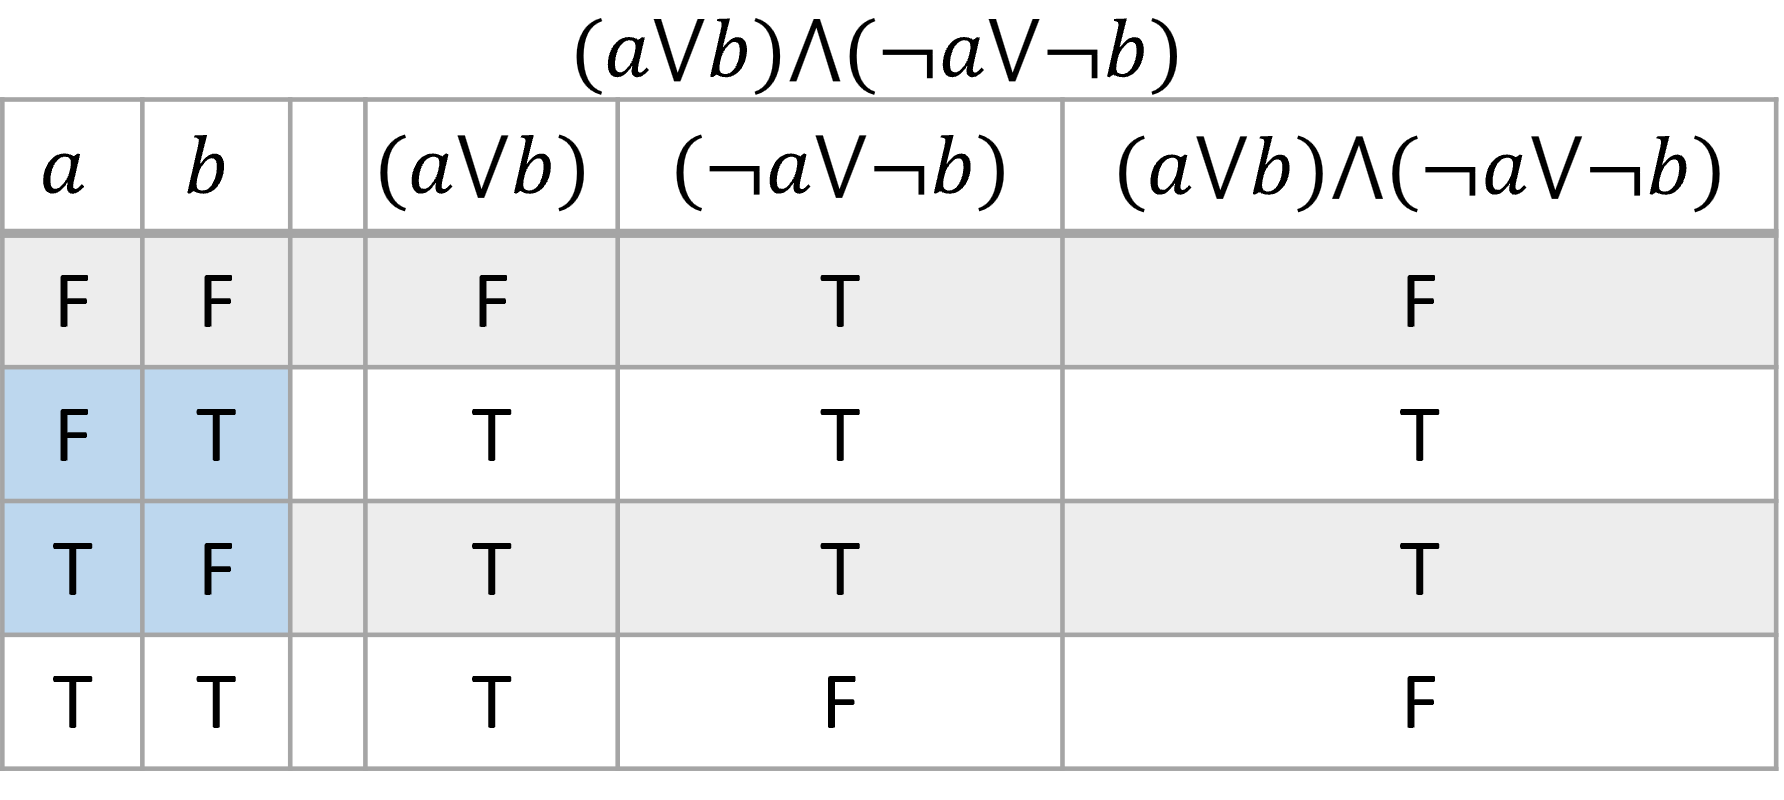
\includegraphics[width=70mm]{figures/sat_example.png}
\end{center}
\caption{Truth Assignment Example with Highlighted Valid Assignment}
\end{figure}

\noindent\rule{4cm}{0.4pt}

\textbf{Wrap Up} 

$\Phi\in $ NP as $\exists$ a verifier $\Psi$ when given an instance $S$ can determine if it is complete/solved in polynomial time, $\Psi\in$ P.

$\Phi\in $ NP-hard as an instance of SAT can be reduced to an instance of 3SAT in polynomial time which can be reduced to an instance of Triangulating a Tripartite Graph in polynomial time which can be reduced to an instance of Latin Square in polynomial time which can be reduced to an instance of Sudoku ($\Phi$) in polynomial time.

As $\Phi\in$ NP and $\Phi\in$ NP-hard, $\Phi\in$ NP-complete. $\square$

Determining if a sudoku grid $p$ has a completion is suspected hard and infeasible for large $n$.

\subsection{Sudoku $\leq_p$ Graph Colouring}

When reducing sudoku to a graph problem the obvious thought is to change it to a graph colouring which is known to be NP-complete. Unfortunately, this is the incorrect reduction direction, while all sudokus can be turned into a graph colouring problem it is not immediately obvious how to change all colouring problems into the input of the sudoku decision problem. 

To transform a grid $p$ to a graph colouring problem:
\begin{itemize}
\item For each cell of the grid create a vertex; $\forall i,j\in D^2$ create vertex $v_{i,j}$, giving $D^4$ vertices in total.
\item Create edges such that: for each $i$ $(v_{i,j},v{i,k})\in E$; for each $j$ $(v_{i,j},v{k,j})\in E$ and for $\lfloor\frac{i-1}{D}\rfloor=\lfloor\frac{k-1}{D}\rfloor$ and $\lfloor\frac{j-1}{D}\rfloor=\lfloor\frac{l-1}{D}\rfloor$, $(v_{i,j},v_{k,l})\in E$.
\item Then for all $D^2$ colours assign a numerical value and for all $S(i,j)\neq 0$ assign the $v_{i,j}$ the colour associated with value $S(i,j)$.
\end{itemize}

Now all sudoku problems can be converted to a $D^2$- colouring problem in polynomial time and since sudoku is NP-complete as long as $D^2$- colouring has a polynomial verifier (which is trivial to check) then it is also NP-complete. 

This emphasises the importance of the reduction direction, it is easy to transform a problem in P to a problem in NP in polynomial time (it is easy to make something more complicated than it needs to be) but the other way round has not yet been done. 

\subsection{Dimension Analysis}

The large string of reductions performed to change a SAT instance into a Sudoku instance can shroud the link between the two as the proofs are somewhat flamboyant. Now to abstract the proofs away and focus on the change in size of the SAT instance to a Sudoku instance. Note that this is not conclusive as from definition of NP-complete class there is multiple ways to create a reduction and one may be more efficient than what has been described, but it is interesting to visit the problem from a view of space complexity (the memory used when computing a result).

A SAT instance with $A$ clauses and $B$ variables is transformed into a 3SAT instance with $A + 3a$ clauses and $B+a$ variables where $a=\Sigma_{c\in C'}|c|-3$, $C'=\{c\in C | |c|>3\}$. 

A 3SAT instance with $C$ clauses and $D$ variables is transformed into a Triangulating a Tripartite Graph instance with $p(D+3C)$ nodes where $p\equiv 0 (\text{mod}3)$.

A Triangulating a Tripartite Graph instance with $E$ nodes is transformed into a Latin Square instance with dimension $\frac{2}{3}E$.

A Latin Square instance with dimension $F$ is transformed into a Sudoku with dimension $F^2$.

In summation, a SAT instance of $A$ clauses and $B$ variables becomes a sudoku instance of dimension $(\frac{2}{3}p(3A+B+10a))^2 $.

\section{Solving Sudoku is Hard}

Decision problems with a boolean yes or no answer have been focused on so far, but, when it comes to being given a sudoku most people assume it is solvable and then search for a solution so a change in perspective to search problems is in order. Is it hard to solve sudoku? 

\begin{equation}
\Gamma(S) = S' \text{ if $\exists$ a completed $S$ else 0}
\end{equation}
Where $S'$ is a completed version of $S$.

It is intuitive that the search problem is harder than the decision problem but let's quantify this into the concepts of P and NP. If $P \neq NP$ then both are infeasible to solve as the search problem is harder than an NP-complete decision problem. However, there is hope hope, if $P=NP$ the corresponding search problem to an NP decision problem $\Gamma$ can be solved in polynomial time. 

\textbf{Theorem}: (from \cite{compcomplexityamodernapproach}) Suppose $P=NP$ then for every problem $\rho\in$ NP there exists a polynomial time Turing Machine $T$ that on input $x$ where $\rho(x)=True$ will output a certificate of $x$.

\textbf{Note:} A certificate in complexity theory refers to a solution path of the decision problem, here it is a completed sudoku grid that is the augmented version of the input. 

\section{Determining Uniqueness is Hard}

\textbf{Def$^n$:} The Sudoku Uniqueness problem is: Given a partially completed sudoku grid $S$ does there exist exactly 1 completion?
\begin{equation}
\Gamma (S) = \begin{cases}
\text{True if only one completion exists} \\
\text{False if multiple completions or none exist}.
\end{cases}
\end{equation}

This decision problem belongs to the class called Difference Polynomial Time (DP or BH$_2$) \cite{dpcomplexity}.

\textbf{Def$^n$:} DP is the class of problems which are the intersection of a problem in NP and a problem in coNP, this is not NP $\cap$ coNP, it is all problems $\Delta$ such that for $a \in $NP and $b\in $coNP:
\begin{equation}
\Delta (x) = \begin{cases}
\text{True if $a(x)$ and $b(x)$ are True} \\
\text{False otherwise }.
\end{cases}
\end{equation}

The definition of $\Gamma$ can be reformulated to immediately show $\Gamma\in$ DP. Instead of saying uniqueness is satisfied by all sudoku grids that have a single solution it can be rephrased to all sudoku grids that have a solution minus all sudoku grids that have at least two solutions; this is the same as $\Delta = \Phi \cap \bar{\Upsilon}$ when $\Upsilon$ is the problem satisfied by sudokus that have at least two solutions. It is known already $\Phi\in$ NP now to show $\Upsilon$ is in NP which is easily done; when given a sudoku and two or more solutions it is easy to verify these separately (as shown in Verification is Easy).$\bar{\Upsilon}$ is satisfied by sudokus with one or no solution and is in coNP by definition. Therefore the intersection of $\Phi$ and $\bar{\Upsilon}$ gives $\Delta$, this formulation is exactly what is needed for $\Gamma\in$ DP.

The complexity of DP is unknown\cite{dphardness}. 

\section{Discussion}
So sudoku is suspected to be hard and all other problems in NP-complete can be reduced to sudoku. This is a great result as it puts a lot of power in the hands of those studying sudoku, as soon as an efficient algorithm is found then all other NP-complete problems can be efficiently solved. Banks and security engineers take advantage of the difficulty of NP-complete problems and use them to encrypt information. So technically as soon as sudoku is efficiently solved banks can be easily robbed and messages on the internet snooped on. But for now this result just means that spending over a day on a sudoku puzzle is justified.
% ~~~~~~~~~~~~~~~~~~~~~~~~~~~~~~~~~~~~~~~~~~~~~~~~~~~~~~~~~~~~~~~~~~~~~~~~~~~~~~~~~~~~~~~~~~~~ %

\chapter{Solving Techniques}
Chapter 2 showed it is hard to solve sudoku, yet a quick google search will yield many websites that do the exactly that. This chapter explores how to go about designing, optimising and ensuring mathematical rigor in the solution algorithms.
\section{Pencil Solutions}
First a human approach to solutions is taken to see if this sheds any light on the problem.

Given an incomplete sudoku puzzle $p\in P_n$ how does one go about completing this.

The easiest technique to observe and implement is coined a \textbf{Forced cell}. Given an empty cell ($p(x,y)=0$) in C$x$ R$y$ B$z$ this cell is forced if the set $F=\{1,...,n\} / \{$ C$x$ $\cup$ R$y$ $\cup$ B$z$ $\}$ has only one element. This is to say $p(x,y)$ has only one valid value other than 0. 

The remining techniques require pencil marks, that is for the average player, notes in each of remaining candidates ($F=\{1,...,n\} / \{$ C$x$ $\cup$ R$y$ $\cup$ B$z$ $\}$), usually only notes if less than 3 or 4 candidates exist. Denote the candidate set for the cell with C$x$ R$y$ B$z$ as $F_{x,y,z}$. $F_{\text{C}x} = \{F_{x,i,j}|i\in\{1,...,n\}, j \in \text{set of boxes C$x$ passes through}\}$, the corresponding definition for $F_{\text{R}x}$ and $F_{\text{B}x}$ applies.

\textbf{Hidden singles}: when a value $v$ appears only in $F_{x,y,z}$ from $F_{\text{C}x}$ (or respectively row or box) this is the only possible place in that column (or row or box) for that value therefore $p(x,y)=v$. This can be extended to doubles, triples etc as when a subset of values of size $m$ occurs in only $m$ sets in $F_{\text{C}x}$ then those candidate cells are reduced to the subset of values.

\textbf{Pointing values}: when a value $v$ appears $F_{\text{B}z}$ (respectively $F_{i,y,z}$) only in sets of form $F_{x,i,z}$ where $i\in \{1,...,n\}$ then all sets in $F_{\text{C}x}/F_{x,i,z}$ must have $v$ eliminated (respectively $F_{\text{R}y}/F_{i,t,z}$). If a candidate value within a box appears only in a single row (or column) then the rest of that row (or column), outside of the box, cannot have that candidate value.

\textbf{X wing}: when a value $v$ appears in four remaining candidate sets such that: two belong to $F_{\text{C}x_1}$, two belong to $F_{\text{C}x_2}$, two belong to $F_{\text{R}y_1}$ and two belong to $F_{\text{R}y_2}$. Then $v$ cannot appear in any other candidate sets for columns C$x_1$, C$x_2$ or rows R$y_1$, R$y_2$. There is a technique called the swordfish that extends this strategy to six cells over the four used here.\footnote{This author recommends the following video by Cracking the Cryptic if one endeavours to learn the X wing technique: https://www.youtube.com/watch?v=gVT786t1Kjk}

\textbf{Y wing}: take a cell at C$x_1$ R$y_1$ with only two remaining candidates, if there exists two more cells with two remaining candidates, one of which is in the first cells remaining candidates, the other being a set value $v$, one belonging to the column of the first cell, the other the row of the first cell(C$x_1$ R$y_2$, C$x_2$ R$y_1$). Then $v$ cannot occur in the remaining candidate set of the cell at C$x_2$ R$y_2$.\footnote{Similarly this author recommends this Cracking the Cryptic video on the Y wing technique: https://www.youtube.com/watch?v=PpHOknAnh4g}

\textbf{Ariadne's thread}\footnote{Named for the mythological Greek princess who helped Theseus escape the maze of the Minotaur by giving him a ball of string allowing him to retrace his steps out of the maze.}: This final technique is one that is difficult for those using pen and paper to implement but is perfect for a computational approach and base the entire solution around this in the next section. Choose the cell with the least amount of elements in its remaining candidate set $F_{x,y,z}$, take the first element $v$ with the set to be the value for $p(x,y)$, work with the above techniques until a contradiction is found (the sudoku board is invalid) and remove $v$ from $F_{x,y,z}$. If no contradiction is found or no technique can be applied to the board it is up to the views of the player when they give up with value $v$. This is ultimately trial and error and is best to leave until last, some may find this an unsatisfying way to solve a sudoku as it lacks the elegance of the other techniques. 

\section{Backtracking}

Ask any computer science student how to solve a sudoku puzzle and the backtracking algorithm will be mentioned within the first breath. One can expect to find this algorithm in a computer science algorithm course as an introduction to recursion, it is not a complex concept and while useful for the usual sizes of newspaper sudoku, as soon as there is an increase to $16 \times 16$ this becomes infeasible. An exploration of this method ensues.

Recursion in terms of computer science is the concept of an algorithm calling itself. As mind bending as a solution using itself as the answer may it can easily be achieved through only two cases. The base case, the smallest version of the problem. And the recursive step, reducing the problem instance to a smaller version of itself. \footnote{The underlying theory of recursion is fascinating and builds on Turing Machines seen previously, see \cite{salomaa1985computation} Chapter 4 for an introduction to the theory.}

One can observe the factorial function ($\Gamma$) as a recursive function. The base case $\Gamma(1)=1$, the recursive step $\Gamma(n)=n\times \Gamma(n-1)$.

The Sierpinski triangle is a more visual version of this, see figure \ref{fig:sieptri}. The base case (when the degree is 1) draws a equilateral triangle of side length $l$. The recursive step is given a length $l$, centre $c$ and a degree $d$. Three versions of itself with degree $d-1$ spawn at the three corners of the triangle for which $c$ is the centre, the corner being the new centre for each and the length is passed as $\frac{l}{2}$.

\begin{figure}[!h]
\begin{center}
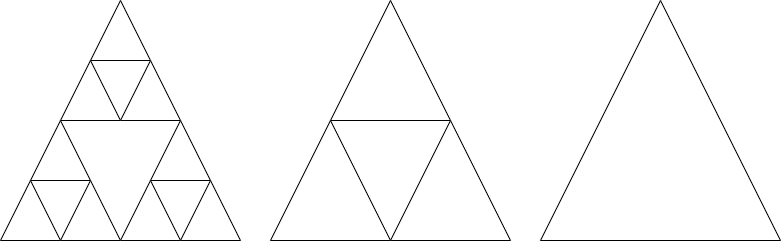
\includegraphics[width=100mm]{figures/SiepTri.png}
\end{center}
\caption{Sierpinski Triangles of degree 3,2 and 1\label{fig:sieptri}}
\end{figure}

How does recursion serve to solve sudoku? Given a sudoku $p$, the base case is a complete sudoku, return the grid if it is valid, otherwise return nothing. The recursive case is where the complexity explodes, if $p$ is of size $n\times n$ and $p(i,j)=0$ for some $(i,j)$ then instantiate $n$ versions of itself each with a $p(i,j)=v$ $\forall v \in \{1,..,n\}$. 

This brute force algorithm is helpful in other ways too, as all combinations of values are tried in each empty cell this can be used to check all option to determine uniqueness by simply adapting the algorithm to count the valids instead of halting.

\begin{algorithm}
\caption{Backtracking}
\begin{algorithmic}
\Procedure{ Backtracking}{grid}
\For {row}
\For {column}
\If{grid(row,column) = 0}
\State{try a value in this position}
\State{Backtracking(grid with new value)}
\If{successful}
\State{return grid}
\Else:
\State{try another value}
\EndIf
\If{no values left to try}
\State{return False}
\EndIf
\EndIf
\EndFor
\EndFor
\State{return grid}
\EndProcedure 
\end{algorithmic}
\end{algorithm}

Why does brute force not work for larger examples? It will work but due to the complexity of the problem it is infeasible, as calculated in chapter 2 the $O(n^{n^2})$ . \footnote{Recursion depth problems may actually impact the brute force algorithm such that it wouldn’t work on any system.}

Many optimisations can be made, and it will be used later on in 6 by 6 enumeration, but it is not a silver bullet, optimisations cannot be continually applied until it is feasible. To get a flavour of what optimisations can be made: only valid values for cell $(i,j)$ cause an instantiation; implementation of the pencil solutions between each cell assignment and even the order of filling in $(i,j)$ can affect run time.

\section{Simulated Annealing} 

If computer scientists were to accept defeat on these NP-complete problems, then many people’s lives would be a lot different. Routing on Google maps certainly would not be available as it is an implementation of a solution to the Travelling Salesman Problem (TSP) $\in$ NP-complete\cite{Applegate2006}. The TSP is a search for the shortest route between two cities. So, there must be a way to solve these problems. Unfortunately, there is no solution so instead there are approximations and stochastic methods. Simulated annealing is the stochastic method studied here but there exist a lot of others that do the same thing in various forms such as A* search \cite{hart1968formal} and the particle swarm optimisation \cite{eberhart1995new}. Simulated annealing stands out from the other methods as it essentially launched the modelling of physical processes as stochastic optimisations. It is named after heat treatment process in metallurgy as this algorithm has a concept of temperature. The algorithm searches a discrete set for a global minimum by escaping local minima through probabilistic methods.

Below is the formulation of the sudoku solving problem in terms of simulated annealing when puzzle $p$ is given.
\begin{itemize}
\item An initial state - $p$ augmented such that $\forall i,j$ where $p(i,j)=0$ reassign so $p(i,j)=x$ where $\forall v \in \{1,...,n\}$ $P(x=v)=\frac{1}{n}$.
\item A finite set - all augmentations of $p$ such that $\forall i,j$ where $p(i,j)\neq0$ the value is unchanged. Call this $S$
\item A cost function J - this will be minimised and therefore must be 0 when the augmentation of p gives a valid sudoku. Here define it as the number of conflicts within a sudoku board. Let $\mathbb{D}=\{1,...,n\}$
\begin{eqnarray}J=&\sum_{i\in\mathbb{D}}\sum_{j\in\mathbb{D}}\sum_{k\in\mathbb{D}/j} \mathbbm{1}\{p(i,j)=p(i,k)\}\\+&\sum_{i\in\mathbb{D}}\sum_{j\in\mathbb{D}}\sum_{k\in\mathbb{D}/i} \mathbbm{1}\{p(i,j)=p(k,j)\}\\+&\sum_{i\in\mathbb{D}}\sum_{j\in\mathbb{D}}\sum_{(k,l)\in\text{B}x/(i,j)} \mathbbm{1}\{p(i,j)=p(k,l)\}\end{eqnarray}
\item A set of neighbours for all $s\in S$. $s_1$ and $s_2$ are neighbours if there is exactly one value pair $(i,j)$ such that $s_1(i,j)=s_2(i,j)$.
\item A cooling schedule $T:\mathbb{N}\rightarrow\mathbb{R}$.
\end{itemize}

The algorithm can be thought of as a markov chain $x(t)$ \cite{simulatedannealing} whose evolution is outlined in algorithm \ref{alg:simann}.

\begin{algorithm}[!h]
\caption{Simulated Annealing\label{alg:simann}\cite{kirkpatrick1983optimization}}
\begin{algorithmic}
\Procedure{SimAnnealing}{$p$, $T$, $J$}
\State{$x(0)=p$}
\For {$i=1 \text{to} \inf$ }
\State{t=T[i]}
\If{$t\leq \epsilon$}
\State{return $x(i)$}
\Else
\State{$n$ = select the neighbour of $x(i)$ randomly}
\If{$J(n) \leq J(x(i))$}
\State{x(i+1) =n }
\Else{ }
\State{$x(i+1) = n $ with probability $e^{-\frac{J(n)-J(x(i))}{t}}$}
\State{$x(i+1)=x(i)$ otherwise}
\EndIf
\EndIf
\EndFor
\EndProcedure
\end{algorithmic}
\end{algorithm}

The main idea of the cooling schedule is to give a high probability of escaping local minima towards the beginning of the runtime and a lower probability towards the end. There exists a lot of room for experimentation within this algorithm as the above formulation can have details changed if the properties remain, these are termed hyperparameters. Many explorations of optimum hyperparameters exist in the literature but there is no decisive method. Currently the formulation has not explicitly defined a cooling schedule so by consulting the literature this can be tuned, from \cite{kirkpatrick1983optimization} for some constant $d$ $T(t)=\frac{d}{\text{log}t}$ is in theory the most popular cooling schedule. 

\subsection{Correctness}
The idea of the algorithm makes intuitive sense, but does it actually produce results and is it better than the brute force solution?

\textbf{Def$^n$}: The optimal set is the set $S^\star$ such that $\forall s \in S^\star$ $J(s)=0$. 

\textbf{Def$^n$}: $s$ communicates with $S^\star$ at height $h$ if $\exists$ a $s,s_1,s_2,...,s_n$ such that $s_i$ and $s_{i+1}$ are neighbours, $s_n\in S^\star$ and $\max_{i\in\{1,...,n\}}(J(s_i))\leq J(s)+h$. 

\textbf{Theorem:} (Hajek, 1988 \cite{sasaki1988time}) Let $d^\star$ be the smallest constant such that $\forall s\in S$ $s$ communicates with $S^\star$ at height $d^\star$, then algorithm \ref{alg:simann} converges if and only if 

\begin{equation}\lim_{t\rightarrow\infty}T(t)=0 \text{ and } \sum^\infty_{t=1}e^{-\frac{d^\star}{T(t)}}=\infty.\end{equation} 

Then by choosing an appropriate $T(t)$ convergence to the optimal set can be ensured, so in theory simulated annealing finds the correct solution. As previously stated $T(t)=\frac{d}{\text{log}t}$ is a popular cooling schedule, this is because if $d\geq d^\star$ then from the theorem simulated annealing converges.

While the algorithm is correct the speed of convergence is not proven to be better than a randomised search of $S$. The only evidence for its use is experimental but with the original paper \cite{kirkpatrick1983optimization} being cited by 27000 papers, according to Google scholar as of April 2023, it is hard to argue with such popularity.

\section{Discussion}

The popular methods of solving sudoku still leave much to be desired. Simulated annealing while not having much mathematical backing the field of stochastic optimisation algorithms still grows. This field is often termed artificial intelligence search leading to the question of whether AI, despite having little mathematical backing, should be used to solve these hard situations. For many the answer is no but for practical applications even if these algorithms do not give exact answers (TSP) they are helpful enough and put us on the right track.

% ~~~~~~~~~~~~~~~~~~~~~~~~~~~~~~~~~~~~~~~~~~~~~~~~~~~~~~~~~~~~~~~~~~~~~~~~~~~~~~~~~~~~~~~~~~~~ %
\chapter{Enumeration is Hard}

Sudoku remains elusive, a good way to generalise solving sudokus without having to throw tonnes of computational power at it has not yet been explored. What if all possible $n$ by $n$ sudokus are stored and loop over these to check if the partially complete sudoku fits into any. Unfortunately, as to be seen in this chapter the amount of sudokus has not been generalised and instead must be calculated or computed on a case by case basis. This is a somewhat disheartening result but luckily there are some fun mathematics than can done along the way to improve efficiency of the calculations and show the need for communication between computers science and mathematics.

\section{Starting Simple - $4 \times 4$}
Let us analyse shidoku the smallest nontrivial sudoku puzzle. Only 2 fundamentally different. One has 96 identical, other has 192. 

\noindent\rule{4cm}{0.4pt}

\textbf{How many Shidoku squares exist?}

$x_4$ is the number of shidoku squares.

First standardise B1 to have ordered cells, 1, 2 on R1, 3,4 on R2. The B1 of any Shidoku square can be transformed to this standardised version through a relabelling (e.g. $1 \mapsto 2$, $2\mapsto 3$ etc). There exists 4! relabelling’s so the amount of Shidoku squares with this standardised B1 is multiplied by 4! to get the true value. Now continue this way until a reasonable search space is reached.

\begin{equation}
x_4 = 4!\times x_a
\end{equation}

\begin{figure}[h]
\centering
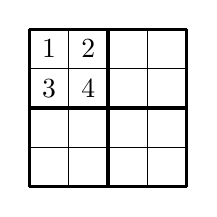
\begin{tikzpicture}[scale=.5]
\begin{scope}
\draw (0, 0) grid (4, 4);
\draw[very thick, scale=2] (0, 0) grid (2, 2);
\setcounter{rowa}{1}
\setrowa {1}{2}{}{}
\setrowa {3}{4}{}{}
\setrowa {}{}{}{}
\setrowa {}{}{}{} 
\end{scope}
\end{tikzpicture}
\caption{B1 standardised}
\label{fig:shidokurelabelling}
\end{figure}

Next set the values for B2 $\cap$ R1. This must be a permutation of $\{3,4\}$, there exists 2! permutations. $x_a = 2\times x_b$. The same applied for B3 $\cap$ C1, permute the set $\{2,4\}$. 

\begin{eqnarray}x_b &= 2\times x_c\\ x_c &=2\times x_d\end{eqnarray}
\begin{figure}[h]
\centering
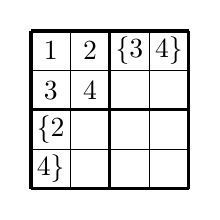
\begin{tikzpicture}[scale=.5]
\begin{scope}
\draw (0, 0) grid (4, 4);
\draw[very thick, scale=2] (0, 0) grid (2, 2);
\setcounter{rowa}{1}
\setrowa {1}{2}{\{3}{4\}}
\setrowa {3}{4}{}{}
\setrowa {\{2}{}{}{}
\setrowa {4\}}{}{}{} 
\end{scope}
\end{tikzpicture}
\caption{Permutations}
\label{fig:shidokupermute}
\end{figure}

The final stage is easy enough to brute force. Observe there exists only three ways to complete the remaining cells.

\begin{figure}[h]
\centering
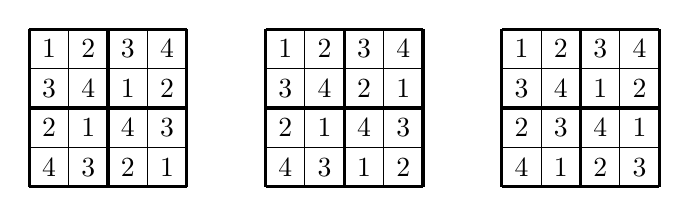
\begin{tikzpicture}[scale=.5]
\begin{scope}[xshift=0cm]
\draw (0, 0) grid (4, 4);
\draw[very thick, scale=2] (0, 0) grid (2, 2);
\setcounter{rowa}{1}
\setrowa {1}{2}{3}{4}
\setrowa {3}{4}{1}{2}
\setrowa {2}{1}{4}{3}
\setrowa {4}{3}{2}{1} 
\end{scope}
\begin{scope}[xshift=6cm]
\draw (0, 0) grid (4, 4);
\draw[very thick, scale=2] (0, 0) grid (2, 2);
\setcounter{rowa}{1}
\setrowa {1}{2}{3}{4}
\setrowa {3}{4}{2}{1}
\setrowa {2}{1}{4}{3}
\setrowa {4}{3}{1}{2} 
\end{scope}
\begin{scope}[xshift=12cm]
\draw (0, 0) grid (4, 4);
\draw[very thick, scale=2] (0, 0) grid (2, 2);
\setcounter{rowa}{1}
\setrowa {1}{2}{3}{4}
\setrowa {3}{4}{1}{2}
\setrowa {2}{3}{4}{1}
\setrowa {4}{1}{2}{3} 
\end{scope}
\end{tikzpicture}
\caption{Three Complete Shidokus}
\label{fig:shidoku}
\end{figure}

This completes the enumeration, there is $x_4=4!\times 2 \times 2 \times 3 = 288$. 

Observe that the last three shidokus squares are not in fact unique, the second transforms to the third. 

\begin{figure}[h]
\centering
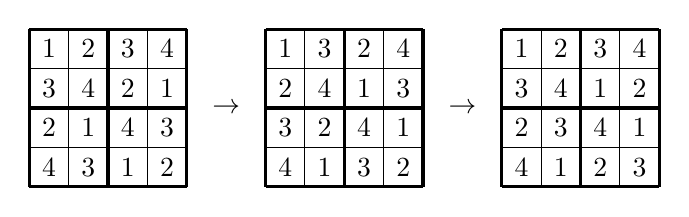
\begin{tikzpicture}[scale=.5]
\begin{scope}
\draw (0, 0) grid (4, 4);
\draw[very thick, scale=2] (0, 0) grid (2, 2);
\setcounter{rowa}{1}
\setrowa {1}{2}{3}{4}
\setrowa {3}{4}{2}{1}
\setrowa {2}{1}{4}{3}
\setrowa {4}{3}{1}{2} 
\end{scope}
\node[anchor=center] at (5, 2) {$\rightarrow$};
\begin{scope}[xshift=6cm]
\draw (0, 0) grid (4, 4);
\draw[very thick, scale=2] (0, 0) grid (2, 2);
\setcounter{rowa}{1}
\setrowa {1}{3}{2}{4}
\setrowa {2}{4}{1}{3}
\setrowa {3}{2}{4}{1}
\setrowa {4}{1}{3}{2} 
\end{scope}
\node[anchor=center] at (11, 2) {$\rightarrow$};
\begin{scope}[xshift=12cm]
\draw (0, 0) grid (4, 4);
\draw[very thick, scale=2] (0, 0) grid (2, 2);
\setcounter{rowa}{1}
\setrowa {1}{2}{3}{4}
\setrowa {3}{4}{1}{2}
\setrowa {2}{3}{4}{1}
\setrowa {4}{1}{2}{3} 
\end{scope}
\end{tikzpicture}
\caption{Transformation}
\label{fig:shidokutransformation}
\end{figure}

Ultimately, there are inly two completely unique shidokus. One of these shidokus has 192 others equivalent and the other 96 this can be seen from the final step of the enumeration, three shidokus are found each with 96 corresponding equivalents but the reduction of three to two shidoku combines the equivalent sets of the two. This shows the amount of equivalent shidokus is dependent on the shidoku square and not all symmetries produce a valid shidoku that hasn't been seen before.

This answered two interesting questions about shidoku through a singular analysis however this will not apply for the larger cases. Instead to generalise this for the unique shidokus the calculation is repeated below with symmetries and equivalence relations as a way to count that is more widely applicable.

\noindent\rule{4cm}{0.4pt}

\textbf{Unique}

Take a group theory approach. Define a Shidoku Symmetry as a map from the set of Shidoku boards to itself. There are two type which to explore. Relabeling symmetries, $x\mapsto y$, change the labels within the shidoku so that all cells with label $x$ change to $y$, set $R_4$ defines all such symmetries. Structural symmetries describe movements of cells, there are many such moves, first all possible symmetries are defined and then condense these into the necessary minimal generators of this set. Name the set $S_4$. The entire set of symmetries is formed from the cartesian product of these sets as they can be combined to get further symmetries (as seen above where sudoku is transformed using a reflection and a relabelling), $G_4=S_4\times R_4$.

Which manipulations of the cells within the Shidoku board map to another valid shidoku board? 
\begin{itemize}
\item Swap R1 and R2,
\item swap R3 and R4,
\item swap C1 and C2,
\item swap C3 and C4,
\item swap S1 and S2,
\item permute T1 and T2,
\item rotate the board 90$^\circ$ clockwise,
\item transpose the board (in the natural way, as though the board were a matrix).
\end{itemize}
Note these structural symmetries are neither extensive (rotations could be included) nor minimal (swapping C1 and C2 can be achieved by rotating, swapping R1 and R2 then rotating 3 more times). Denoting $s$ as the swap of R3 and R4, $r$ the 90$^\circ$ clockwise rotation and $t$ the transpose, $H_4$ can be generated through these.

\begin{equation}H_4 = \langle s,r,t | e=s^2=r^4=t^2\rangle\end{equation}

$G_4$ is of order $128\times 4!=3072$. However, this is much larger than the set of shidoku boards. Note from the previous analysis the largest set of equivalent shidokus is of size 192. This suggests a smaller $G_4$ group can be found as its minimum possible size is 192. \cite{arnold2013minimal} explores the possible minimal groups in detail see table \ref{table:group} for a summary. Finding a minimal symmetry group is not just satisfying but it is useful as it greatly reduces the computation required for the next step.

\begin{table}[!h]
\begin{center}
\begin{tabular}{ |c|c|c| }
\hline
Group & Order & Orbits\\
\hline
$\langle r,t \rangle \times S_4$ & 192 & 5\\
$\langle r,s \rangle \times S_4$ & 1536 & 2\\
$\langle r,s \rangle \times \langle (123)\rangle$ & 192 & 2\\
$\langle s,t \rangle \times S_4$ & 192 & 2\\
$H_4 \times\langle (123) \rangle $ & 384 & 2\\
$\langle r^2,s,t \rangle \times \langle (123) \rangle$ & 192 & 2\\
\hline
\end{tabular}
\end{center}
\caption{\label{table:group}Groups, Order and Orbits}
\end{table}

\textbf{Burnside's Lemma:} For a thorough overview of this result see \cite{jin2018analysis}, an account and analysis that this author found very useful. For a finite group $G=G_4$ acting on the set $S$ of shidoku boards $S/G_4$ denotes the set of orbits of $S$. 
\begin{equation} |S/G_4|=\frac{1}{|G_4|}\sum_{g\in G_4}|S^g|\end{equation}
where $|S^g|$ is the set of all elements in $S$ that are unchanged by element $g$ acting upon it. In English this means orbits (how many distinct shidokus exist) of the shidoku symmetries acting on the set of shidoku boards can be counted by calculating the average of the boards left unchanged by each element of the symmetry group. 

Now to change the idea of equivalence a bit but it will not change its underlying meaning, only the interaction with it. All elements of the symmetry group can be viewed as a structural symmetry action followed by a relabelling action so a board $s\in S$ is invariant if for $g\in S_4$ and $h\in H_4$, $h(g(s))=s$ or $g(s)=h^{-1}(s)$ as $H_4 $ is a group, $h^{-1}\in H_4$. So, with the maths aside invariance can be observed through the lens of just the structural symmetries. A shidoku board $b\in S$ if invariant under structural symmetry $x$ if there exists a relabelling symmetry $r\in R_4$ such that $r$ can undo the action $x$.

Observe to minimise calculations a minimal symmetry group (order 192) is chosen and as the equivalence concept allows focus on the structural symmetries this is minimised. Choose use of $\langle s,t \rangle \times S_4$ from the table \ref{table:group}.

Another way to minimise calculations is to find conjugacy classes, as for conjugacy class C if $a\in C$ and $a$ acting on puzzle B is invariant, that is there exists $r\in R_4$ such that$ra(B)=B$ then all elements conjugate to $a$ such that $b=gag^{-1}$ for $g\in H_4$ are also invariant. This arises from the following, note elements of $R_4$ commute with elements of $H_4$ and from ra(B)=B, $r=a^{-1}$:
\begin{eqnarray}
rb(B)&=&rgag^{-1}(B)\\
&=&grag^{-1}(B)\\
&=&geg^{-1}(B)\\
&=&gg^{-1}(B)\\
&=&e(B)\\
&=&B
\end{eqnarray}
There are five conjugacy classes so only five symmetries should be checked for invariance. 

Prove invariance by considering fixing relationships between structure and relabelling. 

\textbf{The Fixing Lemmas}: If b in S is invariant under x via r then:
\begin{itemize}
\item Value: if a cell location is unchanged under x having value n, r must map $n \mapsto n$.
\item Region: if all cells in a block, sash or pillar are unchanged under x then r is the identity relabeling. 
\item Fixed Point: if r maps $n\mapsto n$ the x must the subset of cells with value n to the same subset.
\end{itemize}
These are easy to verify through observation but if the reader requires a solid proof go to page 10 of \cite{arnold2013minimal}.

Now to calculate the number of orbits through the Burnside Lemma, see table \ref{table:burnside}. A brief discussion: as s fixes R1 and R2 this cannot be invariant as the fixing lemmas suggest $r$ would be the identity relabelling but $s(b)\neq b$; $stst$ fixes B1 so the same reasoning applies. As for $t$, the relabelling must be such that the main diagonal in B1 remains the same (so 1 and 4 are unchanged when the standardised B1 configuration is used) and the other two cells in B1 are flipped ($2\mapsto 4$). Observe in \ref{fig:transpose} there are only two shidoku squares that are invariant under a transpose and the proposed relabelling. The identity element of course preserves all shidoku boards.

\begin{figure}[h]
\centering
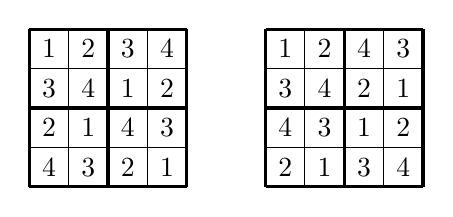
\begin{tikzpicture}[scale=.5]
\begin{scope}[xshift=0cm]
\draw (0, 0) grid (4, 4);
\draw[very thick, scale=2] (0, 0) grid (2, 2);
\setcounter{rowa}{1}
\setrowa {1}{2}{3}{4}
\setrowa {3}{4}{1}{2}
\setrowa {2}{1}{4}{3}
\setrowa {4}{3}{2}{1} 
\end{scope}
\begin{scope}[xshift=6cm]
\draw (0, 0) grid (4, 4);
\draw[very thick, scale=2] (0, 0) grid (2, 2);
\setcounter{rowa}{1}
\setrowa {1}{2}{4}{3}
\setrowa {3}{4}{2}{1}
\setrowa {4}{3}{1}{2}
\setrowa {2}{1}{3}{4} 
\end{scope}
\end{tikzpicture}
\caption{These shidoku are invariant under $t$, $2\mapsto 3$}
\label{fig:transpose}
\end{figure}

\begin{table}[!h]
\begin{center}
\begin{tabular}{ |c|c| }
\hline
Class & No. of Invariant boards\\
\hline
$C_e=\{e\}$&$12\times 4!$\\
$C_s = \{s,tst\}$&0\\
$C_t = \{t,sts\}$&$2\times4!$\\
$C_{st}=\{st,ts\}$&0\\
$C_{stst}=\{stst\}$&0\\
\hline
\end{tabular}
\end{center}
\caption{\label{table:burnside}}
\end{table}

The Burnside lemma gives:
\begin{equation}|S/G_4|=\frac{1(12\times 4!)+ 2(0)+2(2\times 4!)+2(0)+1(0)}{8\times 4!}=2.\end{equation}
To prove what was already known! At least these techniques can be applied to larger boards.

The main issue here of course is fining a minimal symmetry group, luckily this paper addresses it \cite{arnold2013minimal} through considering the structural and relabelling symmetries separately as a helpful technique. 

Now to move on to bigger and better sudokus.

\section{Getting Harder - $6 \times 6$}
Unlike square number sudoku like the $4\times4$ and the $9\times 9$ case there is no in-depth literature on the enumeration of the the $6 \times 6 $ case so this author provides a detailed discussion on an exhaustive enumeration of all sudoku boards along with code and the unique case is outlined.

\noindent\rule{4cm}{0.4pt}

\textbf{How many?}

A similar strategy is followed to count the rudoku boards.

The first move is always the easiest, standardise B1, see figure \ref{fig:61}. Reducing the search space by 9!. $x_6=9!\times x_a$

\begin{figure}[h]
\centering
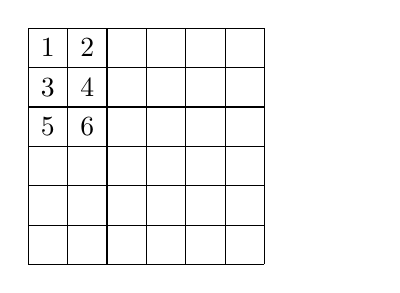
\begin{tikzpicture}[scale=.5]
\begin{scope}[xshift=1.5cm]
\draw (0, 3) grid (6, 9);
\setcounter{row}{1}
\setrow {1}{2}{} {}{}{} {}{}{}
\setrow {3}{4}{} {}{}{} {}{}{}
\setrow {5}{6}{} {}{}{} {}{}{}
\setrow {}{}{} {}{}{} {}{}{}
\setrow {}{}{} {}{}{} {}{}{}
\setrow {}{}{} {}{}{} {}{}{}

\end{scope}
\end{tikzpicture}
\caption{Standardised B1}
\label{fig:61}
\end{figure}

The R1 will be separated into two cases coined pure and mixed. A pure R1 consists of B1 $\cap$ R2 in a single box (B2 $\cap$ R1 or B3 $\cap$ R1) and B1 $\cap$ R3 in the other. A mixed, like the name suggests has B2 $\cap$ R1 as an amalgamation of B1's R2 and R3. The pure case is simple, the first row consists of set $\{3,4\}$ $\{5,6\}$ which forces the sets in R2 and R3, see figure \ref{fig:62}. The count is therefore $2^6$ for the different permutations of these sets multiplied by 2 as B2 and B3 can be permuted. $2^7=128$

\begin{figure}[h]
\centering
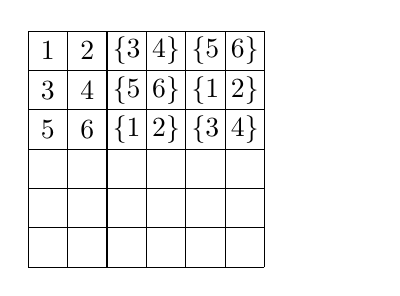
\begin{tikzpicture}[scale=.5]
\begin{scope}[xshift=1.5cm]
\draw (0, 3) grid (6, 9);
\setcounter{row}{1}
\setrow {1}{2}{\{3} {4\}}{\{5}{6\}} {}{}{}
\setrow {3}{4}{\{5} {6\}}{\{1} {2\}}{}{}{}
\setrow {5}{6}{\{1} {2\}}{\{3}{4\}} {}{}{}
\setrow {}{}{} {}{}{} {}{}{}
\setrow {}{}{} {}{}{} {}{}{}
\setrow {}{}{} {}{}{} {}{}{}

\end{scope}
\end{tikzpicture}
\caption{Pure S1}
\label{fig:62}
\end{figure}

Mixed takes more consideration. R1 must be a permutation of sets has two choices $\{\{3,5\},\{4,6\}\}$ or $\{\{3,6\},\{4,5\}\}$. This forces 5,6 to be in R2 and 3,4 into R3 leaving 1,2 to be placed, see figure \ref{fig:63}. Counting these decisions there are 2 for where 1 is placed (forcing 2), 2 for which R1 set take, 2 to flip B2 and B3 then $2^6$ to permute each of the sets. Overall there are $2\times 2 \times 2 \times 2^6=2^9=512$. 

\begin{figure}[h]
\centering
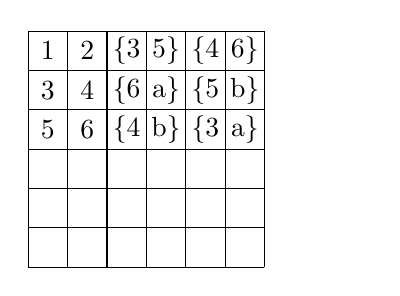
\begin{tikzpicture}[scale=.5]
\begin{scope}[xshift=1.5cm]
\draw (0, 3) grid (6, 9);
\setcounter{row}{1}
\setrow {1}{2}{\{3} {5\}}{\{4}{6\}} {}{}{}
\setrow {3}{4}{\{6} {a\}}{\{5} {b\}}{}{}{}
\setrow {5}{6}{\{4} {b\}}{\{3}{a\}} {}{}{}
\setrow {}{}{} {}{}{} {}{}{}
\setrow {}{}{} {}{}{} {}{}{}
\setrow {}{}{} {}{}{} {}{}{}

\end{scope}
\end{tikzpicture}
\caption{Mixed S1}
\label{fig:63}
\end{figure}

S1 has $2^9+2^7=640$ possible completions. Now count how many S2 completions there are for each board, call this $b_i$.

\begin{equation}x_a = \sum^{640}_{i=1}b_i\end{equation}

This will take a lot of computation power, so it is best to simplify this further. Observe a completion of S1 has the same $b_i$ as the same completion of S1 but with B2 and B3 flipped, currently this is computed twice but this is a waste. Expand this idea further to permutation of R3-4 and R5-6. This means each board in the 640 completions has $2\times 2\times 2$ boards that are equivalent when columns and boxes are permuted. This limits the search space to $\frac{640}{8}=80$. In practise this means choices described above are enforced. For the pure case set R1 to be 1,2,3,4,5,6 leaving only $2^4=16$ choices. Then for the mixed case set R1 to be 1,2,3,5,4,6 or 1,2,3,6,4,5 leaving $2^5$ choices left and remember the choice between these two R1s gets $2^6=64$. 

\begin{equation}x_a=8\sum^{80}_{i=1}b_i\end{equation}

There is still work to be done, for all 80 boards $b_i$ must be computed. First, a brief approximation: for each column in S2 there are three possible numbers this gives $3!^6 = 46656$ possible solutions that need to be checked. Still, this can be reduced further. For C1 $\cup$ S2 set 2,4,6 removing the need to count individually for the 3! permutations as they same number of completions as the board with forced C1, see figure \ref{fig:64}. So, redefine the $b_i$ to count only solutions with C1 1,3,5,2,4,6.

\begin{equation}x_6=9!3!8\sum^{80}_{i=1} b_i\end{equation}

\begin{figure}[h]
\centering
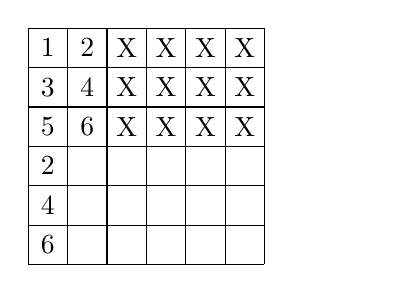
\begin{tikzpicture}[scale=.5]
\begin{scope}[xshift=1.5cm]
\draw (0, 3) grid (6, 9);
\setcounter{row}{1}
\setrow {1}{2}{X} {X}{X}{X} {}{}{}
\setrow {3}{4}{X} {X}{X} {X}{}{}{}
\setrow {5}{6}{X} {X}{X}{X} {}{}{}
\setrow {2}{}{} {}{}{} {}{}{}
\setrow {4}{}{} {}{}{} {}{}{}
\setrow {6}{}{} {}{}{} {}{}{}

\end{scope}
\end{tikzpicture}
\caption{C1 enforced}
\label{fig:64}
\end{figure}

From this authors own computation $\sum^{80}_{i=1} b_i=816$. \footnote{The source code can be found at https://github.com/EveRoutledge/sudoku/66enumeration.py, the code is in python and yet still runs in under a minute.}

Finally, this gives $x_6=28200960$. This does not look promising, there is a massive difference from $x_4=288$.

\noindent\rule{4cm}{0.4pt}

\textbf{Unique}

Leading on from the 4 by 4 approach the following symmetries are observed and are sufficient to generate the group $G_4$.
\begin{itemize}
\item Relabeling,
\item swap R1 and R2, swap R2 and R3, swap R4 and R5, swap R5 and R6,
\item swap C1 and C2, swap C3 and C4, swap C5 and C6
\item swap S1 and S2,
\item swap T1 and T2, swap T2 and T3,
\item rotate the board 180$^\circ$,
\item transpose the board (in the natural way, as though the board were a matrix).
\end{itemize}
The rudoku board requires a different approach to the shidoku mainly as the boxes are not squares. This immediately rules out the transpose of the board and the rotation must be a half turn not just a quarter turn. In fact, this can be reduced further the rotation can be formed from R1-R2, R2-R3, R1-R2, R4-R5, R5-R6, R4-R5, S1-S2, T1-T2, T2-T3, T1-T2, C1-C2, C3-C4, C5-C6. Finally combine C1-C2 and T1-T2 to give C3-C4, this can be expanded to C5-6, R4-R5 and R5-R6.

The $4\times 4$ case emphasised the need for reducing the symmetry group size. However, with many of the efficiencies of the reduction stemming from the transposes ability to transform a column to a row, the same cannot be done here. One efficiency can still be used, by abstracting the relabelling symmetries $R_4$ into the invariance definition. A sudoku board is invariant under $x$ if there exists a relabelling $r$ such that $r=x^{-1}$. 

The group of symmetries is given by $G_6=S_6\times R_6$. To calculate the order of this group it is separated into direct products. 

\begin{equation}
S_6=\langle\text{R1-R2, R2-R3, S1-S2}\rangle\times \langle\text{T1-T2, T2-T3, C1-C2}\rangle 
\end{equation}

The order is: $|S_6|=2(3!)^2\times 2^3(3!) =3456$ multiplied in order of the groups above to allow direct comparison of the group and its order. 

Unfortunately with a group that large the rest of the calculations are tedious in fact from \cite{Jarvis2005} Russell and Jarvis calculated 90 conjugacy classes which is too many to calculate by hand. The rest of the Burnside Lemma calculations again can be viewed here \cite{Jarvis2005}. Spoiler alert: the number of unique $6\times 6$ sudokus is 49.

\section{The Big One - $9 \times 9$}

Now it is time to tackle the big one. The 9 by 9 sudoku is the largest board size for which enumerations have been widely discussed with this author only finding one website discussing the 10 by 10 case. Similarly, enumerations for the Latin square stop at 11. Chapter 2 explored theoretical exponential increase in difficulty when sudoku boards increase in size and this has been seen in action throughout this chapter. A generalised and efficient enumeration method seems unlikely but is certainly fun to attempt so this paper continues to the final enumeration.

\textbf{How many?}

Start as usual by standardising B1. This shrinks the search space by a factor of 9!. Then the usual technique takes place, find all possible S1 configurations, group them into sets that will have the same number of completions for S2 and S3 then brute force the completions with an optimised algorithm.

To calculate the number of possibilities for S1 examine the pure and mixed case. The pure case uses the set in B1 $\cup$ R2 ($\{4,5,6\}$) in either B2 $\cup$ R1 or B3 $\cup$ R1 and B1 $\cup$ R3 ($\{7,8,9\}$) in the other. This forces the sets in the other rows of S1. Counting these gives $3!^6$ for the permutations of each set and as T2 and T3 can be switched multiply by two. There are $2\times 3!^6$ pure cases of S1. 

The mixed case is a little more complicated. First list the possible R1 $\cup$ B2 $\cup$ B3 options, see table \ref{table:mixed99}. This will set three values in the second and three in the third row leaving $\{1,2,3\}$ to be placed in the remaining cells. See figure \ref{fig:91}. Counting these gets $3\times3!^6$ for each configuration of the top row. Finally, there are $9\times 2$ top row configurations from the table selection and by swapping the P2 and P3. 

\begin{table}[!h]
\begin{center}
\begin{tabular}{ |c|c| }
\hline
B2 $\cup$ R1 & B3 $\cup$ R1\\
\hline
$\{4,5,7\}$&$\{6,8,9\}$\\
$\{4,5,8\}$&$\{6,7,9\}$\\
$\{4,5,9\}$&$\{6,7,8\}$\\
$\{4,6,7\}$&$\{5,8,9\}$\\
$\{4,6,8\}$&$\{5,7,9\}$\\
$\{4,6,9\}$&$\{5,7,8\}$\\
$\{5,6,7\}$&$\{4,8,9\}$\\
$\{5,6,8\}$&$\{4,7,9\}$\\
$\{5,6,9\}$&$\{4,7,8\}$\\
\hline
\end{tabular}
\end{center}
\caption{\label{table:mixed99}}
\end{table}
\begin{figure}[h]
\centering
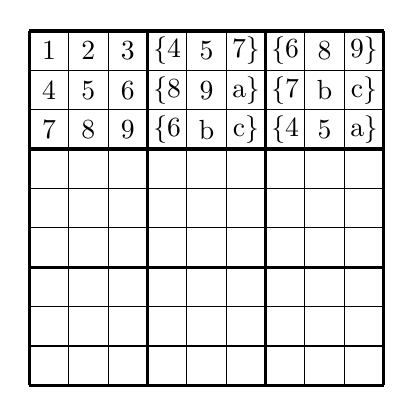
\begin{tikzpicture}[scale=.5]
\begin{scope}[xshift=1.5cm]
\draw (0, 0) grid (9, 9);
\draw[very thick, scale=3] (0, 0) grid (3, 3);
\setcounter{row}{1}
\setrow {1}{2}{3} {\{4}{5}{7\}} {\{6}{8}{9\}}
\setrow {4}{5}{6} {\{8}{9}{a\}} {\{7}{b}{c\}}
\setrow {7}{8}{9} {\{6}{b}{c\}} {\{4}{5}{a\}}
\setrow {}{}{} {}{}{} {}{}{}
\setrow {}{}{} {}{}{} {}{}{}
\setrow {}{}{} {}{}{} {}{}{}
\setrow {}{}{} {}{}{} {}{}{}
\setrow {}{}{} {}{}{} {}{}{}
\setrow {}{}{} {}{}{} {}{}{}

\end{scope}
\end{tikzpicture}
\caption{An example of the mixed R1 case.}
\label{fig:91}
\end{figure}
In total there are
\begin{equation}2\times3!^6+18\times 3\times 3!^6 = 2612736\end{equation}
S1 configurations with the standardised B1. This is an unreasonably large search space so must be reduced like has been done previously through equivalence relations to discover which boards will have the same number of completions. Reductions are explored below.

\textbf{Column Permutations}
Observe boards with different permutations of C4-6 have the same number of completions (see \ref{fig:equiv99}). This is expanded to permutations of C7-9 and B2-3. Therefore from a single board one can derive $3!\times3!\times2=72$ other boards that are essentially equivalent. The search space becomes $\frac{2612736}{72}=36288$, better but not ideal.

\begin{figure}[h!]
\centering
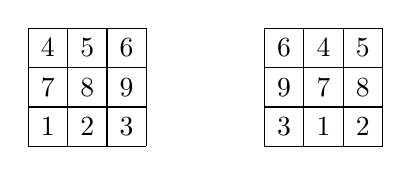
\begin{tikzpicture}[scale=.5]
\begin{scope}[xshift=0cm]
\draw (0, 0) grid (3, 3);
\setcounter{rowb}{1}
\setrowb {4}{5}{6}
\setrowb {7}{8}{9}
\setrowb {1}{2}{3}
\end{scope}
\begin{scope}[xshift=6cm]
\draw (0, 0) grid (3, 3);
\setcounter{rowb}{1}
\setrowb {6}{4}{5}
\setrowb {9}{7}{8}
\setrowb {3}{1}{2}
\end{scope}
\end{tikzpicture}
\caption{\label{fig:equiv99}Two configurations of B2 which are essentially equivalent}
\end{figure}

\textbf{Optimised Column Permutations and Relabelling}
B1 has been excluded in the permutation above in order to preserve the standardised B1 labeling but note relabeling is a symmetry and this can be utilised further to improve the search space ($r_1pr_2$). Permute C1-3, C4-6, C7-9 and B1-3 giving $3!\times 3!\times 3! \times 3!=1296$ possibly equivalent boards to be derived from a single board. Relabel the new boards to again standardise B1. From \cite{felgenhauer2005enumerating} page 4 it is stated this reduces the search space to 2051 boards. If each board had exactly 1296 equivalent boards there would be $\frac{2612736}{1296}= 2016$ boards in the search space. Now to catalogue the number of boards corresponding to each of the 2051 as, unlike the previous reduction, this reduction does not affect all boards equally.

\textbf{Permutations of S1 Rows}
Taking a leaf out of the Optimised Column Permutations and Relabelling book, apply this to the rows of sash 1. Permuting the rows and relabelling B1 to its standardised form. This gives each board another the possibility of having $3!$ more equivalent boards now giving a grand maximum of $1296\times 3!=7776$ equivalent boards, of course this is not the case for every board as discussed, otherwise the search space could have been $\frac{2612736}{7776}=336$ but not far off with the reduction coming out at 416 (from \cite{felgenhauer2005enumerating} page 4).

\textbf{Reducing Twins}
Twins are two values in C$n$ lying in R$x$ and R$y$ such that the values also lie in C$m$ in R$x$ and R$y$ where $n\neq m$. For example figure \ref{fig:twins} has values 1 and 4 in R1, R2, C1, C4. By the relabeling $1\mapsto 4$, $4\mapsto 1$ another board is found with the same number of completions, that is to say the complete S2,3 are independent of the labels 1 and 4. This gives another equivalence reduction. From \cite{felgenhauer2005enumerating}page 5 the 416 equivalence classes reduce to 174.

\begin{figure}[h!]
\centering
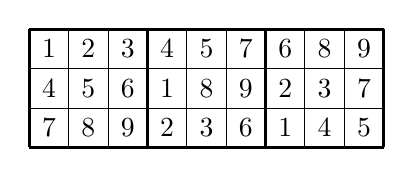
\begin{tikzpicture}[scale=.5]
\begin{scope}[xshift=0cm]
\draw (0, 0) grid (3, 3);
\draw[very thick, scale=3] (0, 0) grid (3, 1);
\setcounter{rowb}{1}
\setrowb {1}{2}{3}
\setrowb {4}{5}{6}
\setrowb {7}{8}{9}
\end{scope}
\begin{scope}[xshift=3cm]
\draw (0, 0) grid (3, 3);
\setcounter{rowb}{1}
\setrowb {4}{5}{7}
\setrowb {1}{8}{9}
\setrowb {2}{3}{6}
\end{scope}
\begin{scope}[xshift=6cm]
\draw (0, 0) grid (3, 3);
\setcounter{rowb}{1}
\setrowb {6}{8}{9}
\setrowb {2}{3}{7}
\setrowb {1}{4}{5}
\end{scope}
\end{tikzpicture}
\caption{\label{fig:twins}}
\end{figure}

Observe this can be expanded to larger subsets of values, see figure \ref{fig:twinsagain} observe 2 and 5 are interchangeable as well as 1 and 4. Again from \cite{felgenhauer2005enumerating} this reduces the equivalence classes to just 71.

\begin{figure}[h!]
\centering
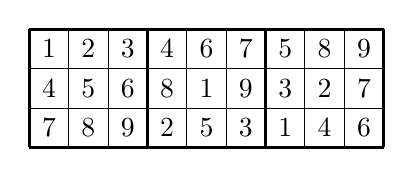
\begin{tikzpicture}[scale=.5]
\begin{scope}[xshift=0cm]
\draw (0, 0) grid (3, 3);
\draw[very thick, scale=3] (0, 0) grid (3, 1);
\setcounter{rowb}{1}
\setrowb {1}{2}{3}
\setrowb {4}{5}{6}
\setrowb {7}{8}{9}
\end{scope}
\begin{scope}[xshift=3cm]
\draw (0, 0) grid (3, 3);
\setcounter{rowb}{1}
\setrowb {4}{6}{7}
\setrowb {8}{1}{9}
\setrowb {2}{5}{3}
\end{scope}
\begin{scope}[xshift=6cm]
\draw (0, 0) grid (3, 3);
\setcounter{rowb}{1}
\setrowb {5}{8}{9}
\setrowb {3}{2}{7}
\setrowb {1}{4}{6}
\end{scope}
\end{tikzpicture}
\caption{\label{fig:twinsagain}}
\end{figure}

Brilliant, S1 has been reduced to only 71 boards to search. However, each class needs to be enumerated which is a lot of searching and as seen in Chapter 2 finding a single solution isn't very efficient so counting how many exist is worse. This search space can be improved by using the exact same argument as S1 on T1 getting 2612736 completions which can be reduced to 36288 equivalence classes with 72 members. Repeat the twins equivalence relation idea but \cite{felgenhauer2005enumerating} reasons the search space has been reduced enough that the computation is feasible.

For algorithmic details consult \cite{felgenhauer2005enumerating}. This paper states the number of valid sudoku grids is
6670903752021072936960, that is 6 sextillion. This has been corroborated by the first discoverer of this number in \cite{lin2004number}.
\noindent\rule{4cm}{0.4pt}
\textbf{Unique} 

To determine the amount of unique sudokus the pattern follows that of the $4\times 4$ and $6\times 6$ case. 

The symmetry group $G_9$ is made up of the usual: relabelling, permuting pillars, sashes, rows and columns, rotations, and a transposition. 

By considering only structural symmetries $S_9$ Russell in \cite{russell2006mathematics} computes a group of size 3359232 with 275 conjugacy classes. 

For the 275 classes fixed point lemmas can be used to reduce this number to 27, again by Russell in \cite{russell2006mathematics}.

This is still going to leave a lot of hand computation so, as becomes second nature in this paper, it is the computers turn. By using a program known as GAP \cite{GAP2021} on a permutation representation of the sudoku symmetries the invariant boards are counted for each conjugacy class. The average of each symmetry's count of invariant boards is taken which by Burnsides Lemma gives us the amount of unique sudoku boards. Russell \cite{russell2006mathematics} states there exist 5472730538 boards.

While this uniqueness counting is not as elegant as those previously recounted, it emphasises the struggle for mathematics to keep up as the sudoku board size grows. The same struggle would be observed in computers if a large enough sudoku board was attempted.

\section{Verification}

Enumerating sudoku requires a computer to work through the laborious and trivial tasks described in this chapter. This is both a strength and a weakness of the computers place in modern mathematics. Previously this work would be inscribed in large notebooks by someone who enjoys monotonous work. Now hundreds of man hours become an hour of coding and pressing run. The improvement is mathematicians are freed up to explore new questions and leave the trivial to the machine, but it also means there is a middle man between the mathematician and the answer, a middle man that may have created errors. Scepticism follows any computational proof, the pure nature of mathematics and logic sullied. This author, straddling the worlds of mathematics and computer science sees the merits of the machine but too feels the lack of satisfaction at the inelegance of the code. 

A famous example of the conflict between mathematics and the computer is the proof of the Four Colour Theorem. The Theorem states: a map requires no more than four colours to colour it in such a way that no adjacent regions have the same colour. The idea of the proof being the mathematicians reduced the map possibilities and a computer then exhausts all possible colourings to confirm each instance only requires four colours. The proof was controversial no person could feasibly check the computation \cite{swart1980philosophical}. The theorem has been proven three times\cite{appel1989every}\cite{BarNatan1996LieAA}\cite{gonthier2008formal}, all using a computer, the most recent of which uses software specifically designed to assist with proving theorems, much like the GAP software used for the sudoku proofs. 

The literature on enumeration of sudokus answers this computer-based scepticism with a complete mathematical proof outline in the works by Jones, Perkins, and Roach \cite{mima2013number} where a formula is given to enumerate $n$ by $n$ sudokus by enumerating the number of reduced sudoku. Further work by Jones, Perkins, and Roach \cite{jones2014number} provides a completely mathematical calculation of the $6\times6$ sudoku.

\section{Discussion}

If the reader remained unconvinced that sudoku is hard from the chapter on NP-completeness, then this chapter providing concrete numbers on the exponential increase of the amount of sudoku grids will hopefully persuade the reader of the seemingly non generalisable puzzle that is sudoku. The sequence of enumerations starts: 288, 28200960, 29136487207403520 \cite{oeis_a291187} , 6670903752021072936960. It is easy to see these increases rapidly.

While it does not seem to be coming any time soon, an exploration of the 12 by 12 case will prove interesting as there exist two factorisations $P_{2,6}$ and $P_{3,4}$. The comparison between these and determining which has more enumerations is not intuitive and to shed light on this is intriguing. The same applied to the 16 by 16 puzzle but with the added bonus of comparing a grid allowing for transposes the $P_{16}$ and one that does not $P_{2,8}$.

As far as a generalised method goes, first standardise B1, categorise R1 into pure and mixed, count how many S1 exist, standardise C1, then enumerate using an optimised backtracking. The unique case is a lot less simple and requires a categorisation of the symmetries, then group into conjugacy classes, determine how many boards the conjugacy class fixes then apply burnside lemma, use of GAP can simplify this.

% ~~~~~~~~~~~~~~~~~~~~~~~~~~~~~~~~~~~~~~~~~~~~~~~~~~~~~~~~~~~~~~~~~~~~~~~~~~~~~~~~~~~~~~~~~~~~ %
\chapter{Conclusion}
\section{Further Work}

Throughout this paper it has been discussed that determining if a sudoku solution exists, solving sudoku, determining the uniqueness of a sudoku and enumerating the number of grids for a given size are all difficult and seemingly impossible to generalise questions within sudoku. Other natural questions fall to the same fate such as the minimum clue question. How many clues must a $n\times n$ sudoku have to have a unique solution? The answer for the $9\times 9$ was recently determined as 17 in \cite{mcguire2014there} and as usual required many computational hours.

As this paper has been algorithm heavy it is interesting to note that sudoku generation techniques are also a large area of theory as algorithms must account for aesthetics (most hobbyists like their sudokus to have rotational symmetry) and difficulty \cite{maji2016comprehensive}. Given all boards can be generated through a backtracking algorithm one would assume it is simply a case of removing cells, however, this does not necessarily preserve uniqueness.

Along the lines of uniqueness another interesting variant of the sudokus came up, the Greco-Latin sudoku squares. These puzzles have two sudokus embedded on top of each with a different alphabet such that each pair of symbols only appears once. Pairs of sudoku boards that can form a Greco-Latin square are termed orthogonal to one another. Interestingly a $6\times 6$ case does not exist \cite{tarry1900probleme}.

The literature of sudoku is expansive and yet tells a similar tale. Generalisable theorems for sudoku may not exist, but one must not stop dreaming.
\section{Closing}

To conclude, sudoku is a brilliant example of a simple game with fascinating mathematics behind it. By embracing the conjunction of mathematics and computation some of the open problems within the field may be solved very soon but it is likely that unless a proof to the P=NP conjecture is found the answers for generalised and large sudoku boards will go on unanswered.


% ~~~~~~~~~~~~~~~~~~~~~~~~~~~~~~~~~~~~~~~~~~~~~~~~~~~~~~~~~~~~~~~~~~~~~~~~~~~~~~~~~~~~~~~~~~~~ %
\bibliographystyle{plain}
\bibliography{refs}
\end{document}

